%% (Master) Thesis template
% Template version used: v2
%
% Largely adapted from Adrian Nievergelt's template for the ADPS
% (lecture notes) project.

%% We use the memoir class because it offers many easy to use features.
% Template v2 fixes:
% Removed titlepage from options: LaTeX Warning: Unused global option(s): [titlepage].
% Electronic version that does not waste space
% \documentclass[11pt,a4paper,openany,oneside]{memoir}
% Printable version that does waste space (but people like it), uncomment for printing
\documentclass[11pt,a4paper]{memoir}

%% Packages
%% ========

%% LaTeX Font encoding -- DO NOT CHANGE
\usepackage[OT1]{fontenc}
\usepackage{subcaption}
\usepackage{float}
\usepackage{algorithm}
\usepackage{algpseudocode}
%% Babel provides support for languages.  'english' uses British
%% English hyphenation and text snippets like "Figure" and
%% "Theorem". Use the option 'ngerman' if your document is in German.
%% Use 'american' for American English.  Note that if you change this,
%% the next LaTeX run may show spurious errors.  Simply run it again.
%% If they persist, remove the .aux file and try again.
\usepackage[english]{babel}

%% Input encoding 'utf8'. In some cases you might need 'utf8x' for
%% extra symbols. Not all editors, especially on Windows, are UTF-8
%% capable, so you may want to use 'latin1' instead.
\usepackage[utf8]{inputenc}

%% This changes default fonts for both text and math mode to use Herman Zapfs
%% excellent Palatino font.  Do not change this.
\usepackage[sc]{mathpazo}

%% The AMS-LaTeX extensions for mathematical typesetting.  Do not
%% remove.
\usepackage{amsmath,amssymb,amsfonts,mathrsfs}

%% NTheorem is a reimplementation of the AMS Theorem package. This
%% will allow us to typeset theorems like examples, proofs and
%% similar.  Do not remove.
%% NOTE: Must be loaded AFTER amsmath, or the \qed placement will
%% break
\usepackage[amsmath,thmmarks]{ntheorem}

%% LaTeX' own graphics handling
\usepackage{graphicx}

%% We unfortunately need this for the Rules chapter.  Remove it
%% afterwards; or at least NEVER use its underlining features.
\usepackage{soul}

%% This allows you to add .pdf files. It is used to add the
%% declaration of originality.
\usepackage{pdfpages}

\usepackage{minted}

%% Some more packages that you may want to use.  Have a look at the
%% file, and consult the package docs for each.
%% See the TeXed file for more explanations

%% [OPT] Multi-rowed cells in tabulars
%\usepackage{multirow}

%% Make document internal hyperlinks wherever possible. (TOC, references)
%% This MUST be loaded before cleveref
\usepackage[linkcolor=black,colorlinks=true,citecolor=black,filecolor=black]{hyperref}

%% [REC] Intelligent cross reference package. This allows for nice
%% combined references that include the reference and a hint to where
%% to look for it.
%% Template v2: cleveref already recognizes what is being referenced - one does not need to write Fig./Sec.
% \usepackage{varioref}. Capitalization is prefered in CS
\usepackage[capitalise]{cleveref}

%% [OPT] Easily changeable quotes with \enquote{Text}
\usepackage[german=swiss]{csquotes}

%% Template v2: this prevents warning "Package fmtcount Warning: \ordinal already defined use \FCordinal instead. on input line". See https://tex.stackexchange.com/questions/162353/memoir-class-conflict-with-datetime#comment371926_162358
\let\ordinal\relax
%% [REC] Format dates and time depending on locale
\usepackage{datetime}

%% [OPT] Provides a \cancel{} command to stroke through mathematics.
%\usepackage{cancel}

%% [NEED] This allows for additional typesetting tools in mathmode.
%% See its excellent documentation.
\usepackage{mathtools}

%% [ADV] Conditional commands
%\usepackage{ifthen}

%% [OPT] Manual large braces or other delimiters.
%\usepackage{bigdelim, bigstrut}

%% [REC] Alternate vector arrows. Use the command \vv{} to get scaled
%% vector arrows.
\usepackage[h]{esvect}

%% [NEED] Some extensions to tabulars and array environments.
\usepackage{array}

%% [OPT] Postscript support via pstricks graphics package. Very
%% diverse applications.
%\usepackage{pstricks,pst-all}

%% [?] This seems to allow us to define some additional counters.
%\usepackage{etex}

%% [ADV] XY-Pic to typeset some matrix-style graphics
%\usepackage[all]{xy}

%% [OPT] This is needed to generate an index at the end of the
%% document.
%\usepackage{makeidx}

%% [OPT] Fancy package for source code listings.  The template text
%% needs it for some LaTeX snippets; remove/adapt the \lstset when you
%% remove the template content.
\usepackage{listings}
\lstset{language=TeX,basicstyle={\normalfont\ttfamily}}

% Template v2 fixes: this is an old package, microtype is superior + fixes an error
%% [REC] Fancy character protrusion.  Must be loaded after all fonts.
\usepackage[activate]{microtype}
% \usepackage[activate]{pdfcprot}  % causes the compilation error

%% [REC] Nicer tables.  Read the excellent documentation.
\usepackage{booktabs}


%% Our layout configuration.  DO NOT CHANGE.
%% Memoir layout setup

%% NOTE: You are strongly advised not to change any of them unless you
%% know what you are doing.  These settings strongly interact in the
%% final look of the document.

% Dependencies
\usepackage{eth-template/ETHlogo}

% Turn extra space before chapter headings off.
\setlength{\beforechapskip}{0pt}

\nonzeroparskip
\parindent=0pt
\defaultlists

% Chapter style redefinition
\makeatletter

\if@twoside
  \pagestyle{Ruled}
  \copypagestyle{chapter}{Ruled}
\else
  \pagestyle{ruled}
  \copypagestyle{chapter}{ruled}
\fi
\makeoddhead{chapter}{}{}{}
\makeevenhead{chapter}{}{}{}
\makeheadrule{chapter}{\textwidth}{0pt}
\copypagestyle{abstract}{empty}
\copypagestyle{something}{empty}


\makechapterstyle{bianchimod}{%
  \chapterstyle{default}
  \renewcommand*{\chapnamefont}{\normalfont\Large\sffamily}
  \renewcommand*{\chapnumfont}{\normalfont\Large\sffamily}
  \renewcommand*{\printchaptername}{%
    \chapnamefont\centering\@chapapp}
  \renewcommand*{\printchapternum}{\chapnumfont {\thechapter}}
  \renewcommand*{\chaptitlefont}{\normalfont\huge\sffamily}
  \renewcommand*{\printchaptertitle}[1]{%
    \hrule\vskip\onelineskip \centering \chaptitlefont\textbf{\vphantom{gyM}##1}\par}
  \renewcommand*{\afterchaptertitle}{\vskip\onelineskip \hrule\vskip
    \afterchapskip}
  \renewcommand*{\printchapternonum}{%
    \vphantom{\chapnumfont {9}}\afterchapternum}}

% Use the newly defined style
\chapterstyle{bianchimod}

\setsecheadstyle{\Large\bfseries\sffamily}
\setsubsecheadstyle{\large\bfseries\sffamily}
\setsubsubsecheadstyle{\bfseries\sffamily}
\setparaheadstyle{\normalsize\bfseries\sffamily}
\setsubparaheadstyle{\normalsize\itshape\sffamily}
\setsubparaindent{0pt}

% Set captions to a more separated style for clearness
\captionnamefont{\sffamily\bfseries\footnotesize}
\captiontitlefont{\sffamily\footnotesize}
\setlength{\intextsep}{16pt}
\setlength{\belowcaptionskip}{1pt}

% Set section and TOC numbering depth to subsection
\setsecnumdepth{subsection}
\settocdepth{subsection}

%% Titlepage adjustments
\pretitle{\vspace{0pt plus 0.7fill}\begin{center}\HUGE\sffamily\bfseries}
\posttitle{\end{center}\par}
\preauthor{\par\begin{center}\let\and\\\Large\sffamily}
\postauthor{\end{center}}
\predate{\par\begin{center}\Large\sffamily}
\postdate{\end{center}}

\def\@advisors{}
\newcommand{\advisors}[1]{\def\@advisors{#1}}
\def\@department{}
\newcommand{\department}[1]{\def\@department{#1}}
\def\@thesistype{}
\newcommand{\thesistype}[1]{\def\@thesistype{#1}}

\renewcommand{\maketitlehooka}{\noindent\ETHlogo[2in]}

\renewcommand{\maketitlehookb}{\vspace{1in}%
  \par\begin{center}\Large\sffamily\@thesistype\end{center}}

\renewcommand{\maketitlehookd}{%
  \vfill\par
  \begin{flushright}
    \sffamily
    \@advisors\par
    \@department, ETH Z\"urich
  \end{flushright}
}

\checkandfixthelayout

\setlength{\droptitle}{-48pt}

\makeatother

% This defines how theorems should look. Best leave as is.
\theoremstyle{plain}
\setlength\theorempostskipamount{0pt}

%%% Local Variables:
%%% mode: latex
%%% TeX-master: "thesis"
%%% End:


%% Theorem environments.  You will have to adapt this for a German
%% thesis.
%% Theorem-like environments

%% This can be changed according to language. You can comment out the ones you
%% don't need.

\numberwithin{equation}{chapter}

%% German theorems
%\newtheorem{satz}{Satz}[chapter]
%\newtheorem{beispiel}[satz]{Beispiel}
%\newtheorem{bemerkung}[satz]{Bemerkung}
%\newtheorem{korrolar}[satz]{Korrolar}
%\newtheorem{definition}[satz]{Definition}
%\newtheorem{lemma}[satz]{Lemma}
%\newtheorem{proposition}[satz]{Proposition}

%% English variants
\newtheorem{theorem}{Theorem}[chapter]
\newtheorem{example}[theorem]{Example}
\newtheorem{remark}[theorem]{Remark}
\newtheorem{corollary}[theorem]{Corollary}
\newtheorem{definition}[theorem]{Definition}
\newtheorem{lemma}[theorem]{Lemma}
\newtheorem{proposition}[theorem]{Proposition}

%% Proof environment with a small square as a "qed" symbol
\theoremstyle{nonumberplain}
\theorembodyfont{\normalfont}
\theoremsymbol{\ensuremath{\square}}
\newtheorem{proof}{Proof}
%\newtheorem{beweis}{Beweis}


%% Helpful macros.
%% Custom commands
%% ===============

%% Special characters for number sets, e.g. real or complex numbers.
\newcommand{\C}{\mathbb{C}}
\newcommand{\K}{\mathbb{K}}
\newcommand{\N}{\mathbb{N}}
\newcommand{\Q}{\mathbb{Q}}
\newcommand{\R}{\mathbb{R}}
\newcommand{\Z}{\mathbb{Z}}
\newcommand{\X}{\mathbb{X}}

%% Fixed/scaling delimiter examples (see mathtools documentation)
\DeclarePairedDelimiter\abs{\lvert}{\rvert}
\DeclarePairedDelimiter\norm{\lVert}{\rVert}

%% Use the alternative epsilon per default and define the old one as \oldepsilon
\let\oldepsilon\epsilon
\renewcommand{\epsilon}{\ensuremath\varepsilon}

%% Also set the alternate phi as default.
\let\oldphi\phi
\renewcommand{\phi}{\ensuremath{\varphi}}


%% use code instead of texttt
\newcommand{\code}[1]{\texttt{#1}}

% Template v2: BibLaTeX with Biber backend are in my opinion best maintainable citation configurations. IEEE style is common in CS.
% Bibliography
\usepackage[
bibstyle=ieee,
citestyle=numeric,
isbn=true,
doi=true,
sorting=none,
url=true,
% defernumbers=true,
bibencoding=utf8,
backend=biber
]{biblatex} %Imports BibLaTeX package
\addbibresource{refs.bib} %Import the bibliography file

%% Document information
%% ====================

\title{Exploring the Correlation between Transactional Bugs and Isolation Levels}
\author{Theodor Moroianu}
\thesistype{Master Thesis}
\advisors{Advisors: Prof.\ Dr.\ David Basin, Dr.\ Si Liu}
\department{Department of Computer Science}
\date{December 3, 2024}


\definecolor{bg}{rgb}{0.95,0.95,0.95}

\begin{document}

\frontmatter

%% Title page is autogenerated from document information above.  DO
%% NOT CHANGE.
\begin{titlingpage}
  \calccentering{\unitlength}
  \begin{adjustwidth*}{\unitlength-24pt}{-\unitlength-24pt}
    \maketitle
  \end{adjustwidth*}
\end{titlingpage}

%% The abstract of your thesis.  Edit the file as needed.
\begin{abstract}

This thesis aims to uncover potential correlations between transactional

%   This thesis aims to understand different trade-offs between current distributed transaction protocols. Specifically, we focus on two widely used concurrency control levels: Causal Consistency and Snapshot Isolation. 

%   First, we aim to understand the different trade-offs between theoretical impossibility results under Causal Consistency: SNOW, NOCS, and NOC-NOC. NOC-NOC is a state-of-the-art concurrency control impossibility result. There are algorithms guided by NOC-NOC. The fundamental rationale behind these algorithms is to move the burdens from the network communication side to the local computation side. We thus conjecture that there are corner cases when local computation itself becomes the new system bottleneck, and thus algorithms guided by NOC-NOC will become sub-optimal. We experiment with a wide range of experiment settings, and the results show that the above conjecture does not hold. The possible explanation is that under current hardware settings, the network communication is much slower than the local computation, and moving the system burden to the local computation is generally a wise choice.


% Second, we focus on improving the efficiency of distributed concurrency control of Snapshot Isolation practically. The key idea behind our protocol is that as the current hardware improves, transactions will practically satisfy the snapshot isolation guarantee in most cases. Many existing protocols incur too much overhead checking whether transactions satisfy the snapshot isolation conditions. Our experiments show that our new distributed snapshot isolation protocols outperform the state-of-the-art.
  
\end{abstract}

\newpage

\section*{Acknowledgement}
TODO: Change.
I am incredibly grateful for having the opportunity to do my master's thesis in the Information Security Group. First and foremost, I would like to express my deepest thanks to Prof. Dr. David Basin. I am also profoundly grateful to my advisor, Dr. Si Liu, for the time we spent discussing the project's progress. I thank him for so many valuable suggestions and advice he gave to me. My master's thesis was partly built on Luca Multazzu's previous master's thesis. I thank him for his detailed help. Although he already left ETH and started to work, he always found a way to accommodate my request.
Without their help, this master's thesis would not be available, and I always owe them a big thank. 


Life at ETH is not always easy. Fortunately, I have many friends with whom I can get through this. I thank Tianqi Chen for always comforting me when I am struggling with difficulties and for spending hours discussing ways to overcome them. I thank Chenhao Li and Yidan Gao for the many jokes they have brought to me, and they have made my life much happier than it would have been. I thank Tao Sun for discussing so many exciting machine learning  problems with me. 

Finally, I would like to express my deepest gratitude to my family. I am always indebted to your unconditional love and support for every decision I made. I thank my parents for supporting me the life at ETH, and for always encouraging me to do what I want to do, for persuading me that I can do anything, for giving me the best quality of life they can. I also thank my wife, Yucheng He, for always listening and talking to me during my most difficult times and for always giving me unconditional love and support.


% \newpage
{\centering
\textit{To my wife Yucheng He and to my parents Yumin Li and Jian Sun}}.
% \



%% TOC with the proper setup, do not change.
\cleartorecto
\tableofcontents
\mainmatter

%% Your real content!
% Some commands used in this file
\newcommand{\package}{\emph}

\chapter{Introduction}
\label{chap:introduction}
\section{Problems and Motivations}

Concurrency control is one of the most important properties in distributed systems and is widely studied. 
There are numerous efforts that are trying to make concurrency control algorithms running efficiently \cite{bernstein1981concurrency, du2013clock, liu2024noc, lu2016snow, thomasian1998concurrency, barghouti1991concurrency, harding2017evaluation, agrawal1987concurrency,lora,ua}. There are different concurrency control levels. The most strict level of concurrency control is strict serializability. Generally speaking, the more rigorous a concurrency level is, the slower the overall performance. Still, it will be much easier for the programmer to understand and reason the system behavior. Increasing the performance of the core concurrency control algorithms will be one of the most crucial factors in improving overall distributed systems performance, such as distributed databases \cite{harding2017evaluation, agrawal1987concurrency}.  


There are two flavors of research in the concurrency control community. The first one focuses more on the theoretical side. More specifically, many research efforts have been devoted to discovering impossibility results between different properties \cite{liu2024noc, lu2016snow}.  The other flavor of the concurrency control community focuses more on the practical side and tries to improve the actual performance of different concurrency control algorithms.


In this project, we mainly focus on three concurrency control levels: strict serializability, snapshot isolation, and causal consistency. Strict serializability is the most strict concurrency control level and performs worst. However, it is easy for programmers to program strictly serializable distributed systems because it is essentially the same as a single-threaded program.  Snapshot isolation is a balance between strict levels and performance. It can avoid most abnormal behaviors but can still achieve pretty decent performance. Lastly, causal consistency is mainly used in web applications where performance is critical.


\paragraph{Problems and Motivations}
We mainly focus on the snapshot isolation concurrency control level because it is one of the most widely used concurrency control levels in practice. We aim to understand impossibility results and improve the practical performance of snapshot isolation concurrency control algorithms. The motivation of the paper is to try to bridge the gap between theoretical impossibility results and practical snapshot isolation concurrency control algorithms.


\section{Contributions}
Overall, we make the following contributions in this project.

\begin{enumerate}
    \item We compare several impossibility results. More specifically, we compare \textbf{NOC-NOC} with other impossibility results to see whether \textbf{NOC-NOC} is always optimal.
    \item We run experiments to validate that there is no bottleneck shift in \textbf{NOC-NOC}.
    \item We propose a practical snapshot isolation concurrency control algorithm based on \cite{lu2023ncc}.
    \item We implement the algorithm and three other baselines.
    \item We compare our practical snapshot isolation algorithm with three other baselines. Experiment results show that our algorithms outperform three other baselines under low contention scenarios.
\end{enumerate}
% This is version \verb-v1.4- of the template.

% We assume that you found this template on our institute's website, so
% we do not repeat everything stated there.  Consult the website again
% for pointers to further reading about \LaTeX{}.  This chapter only
% gives a brief overview of the files you are looking at.

% \section{Features}
% \label{sec:features}

% The rest of this document shows off a few features of the template
% files.  Look at the source code to see which macros we used!

% The template is divided into \TeX{} files as follows:
% \begin{enumerate}
% \item \texttt{thesis.tex} is the main file.
% \item \texttt{extrapackages.tex} holds extra package includes.
% \item \texttt{layoutsetup.tex} defines the style used in this document.
% \item \texttt{theoremsetup.tex} declares the theorem-like environments.
% \item \texttt{macrosetup.tex} defines extra macros that you may find
%   useful.
% \item \texttt{introduction.tex} contains this text.
% \item \texttt{sections.tex} is a quick demo of each sectioning level
%   available.
% \item \texttt{refs.bib} is an example bibliography file.  You can use
%   Bib\TeX{} to quote references.  For example, read the book from
%   Bringhurst~\cite{bringhurst1996ets} if you can get a hold of it.
  
%   If you need to refer to multiple authors without wanting to name them,
%   you can refer to an article by Einstein et al.~\cite{einstein1935can}.
  
%   Note that the tilde sign $\sim$ between the name and citation is
%   necessary to prevent any unwanted breakage.
% \end{enumerate}


% \subsection{Extra package includes}

% The file \texttt{extrapackages.tex} lists some packages that usually
% come in handy.  Simply have a look at the source code.  We have
% added the following comments based on our experiences:
% \begin{description}
% \item[REC] This package is recommended.
% \item[OPT] This package is optional.  It usually solves a specific
%   problem in a clever way.
% \item[ADV] This package is for the advanced user, but solves a problem
%   frequent enough that we mention it. Consult the package's
%   documentation.
% \end{description}

% As a small example, here is a reference to the Section \emph{Features}
% typeset with the recommended \package{cleveref} package:
% \begin{quote}
%   See \cref{sec:features}.
% \end{quote}


% \subsection{Layout setup}

% This defines the overall look of the document -- for example, it
% changes the chapter and section heading appearance.  We consider this
% a `do not touch' area.  Take a look at the excellent \emph{Memoir}
% documentation before changing it.

% In fact, take a look at the excellent \emph{Memoir} documentation,
% full stop.


% \subsection{Theorem setup}

% This file defines a bunch of theorem-like environments.

% \begin{theorem}
%   An example theorem.
% \end{theorem}

% \begin{proof}
%   Proof text goes here.
% \end{proof}

% Note that the q.e.d.\ symbol moves to the correct place automatically
% if you end the proof with an \texttt{enumerate} or
% \texttt{displaymath}.  You do not need to use \verb-\qedhere- as with
% \package{amsthm}.

% \begin{theorem}[Some Famous Guy]
%   Another example theorem.
% \end{theorem}

% \begin{proof}
%   This proof
%   \begin{enumerate}
%   \item ends in an enumerate.
%   \end{enumerate}
% \end{proof}

% \begin{proposition}
%   Note that all theorem-like environments are by default numbered on
%   the same counter.
% \end{proposition}

% \begin{proof}
%   This proof ends in a display like so:
%   \begin{displaymath}
%     f(x) = x^2.
%   \end{displaymath}
% \end{proof}


% \subsection{Macro setup}

% For now the macro setup only shows how to define some basic macros,
% and how to use a neat feature of the \package{mathtools} package:
% \begin{displaymath}
%   \abs{a}, \quad \abs*{\frac{a}{b}}, \quad \abs[\big]{\frac{a}{b}}.
% \end{displaymath}

\input{Background}
\chapter{Developping a DBMS Transactional Testing Framework}

\section{Overview}

This chapter presents the design, implementation and usage of a testing framework for replicating DBMS transactional bugs. Using the testing framework, we replicate a set of transactional bugs in the \textit{MySQL}, \textit{MariaDB} and \textit{TiDB} DBMSs. We then analyse the reports of the replicated bugs, and we explore the corelation between isolation levels and the reported bugs.

\section{Design}

The testing framework, is implemented in \textit{Python}, and heavily relies on \textit{Podman}, a container manager \cite{podmanwebpage} for managing DBMS instances. The tool works on \code{x64 GNU/Linux} systems, and we developped it in \textit{VSCode}, with the help of \textit{Github Copilot} \cite{copilotwebpage}.


\begin{figure}[!h]
    \centering
    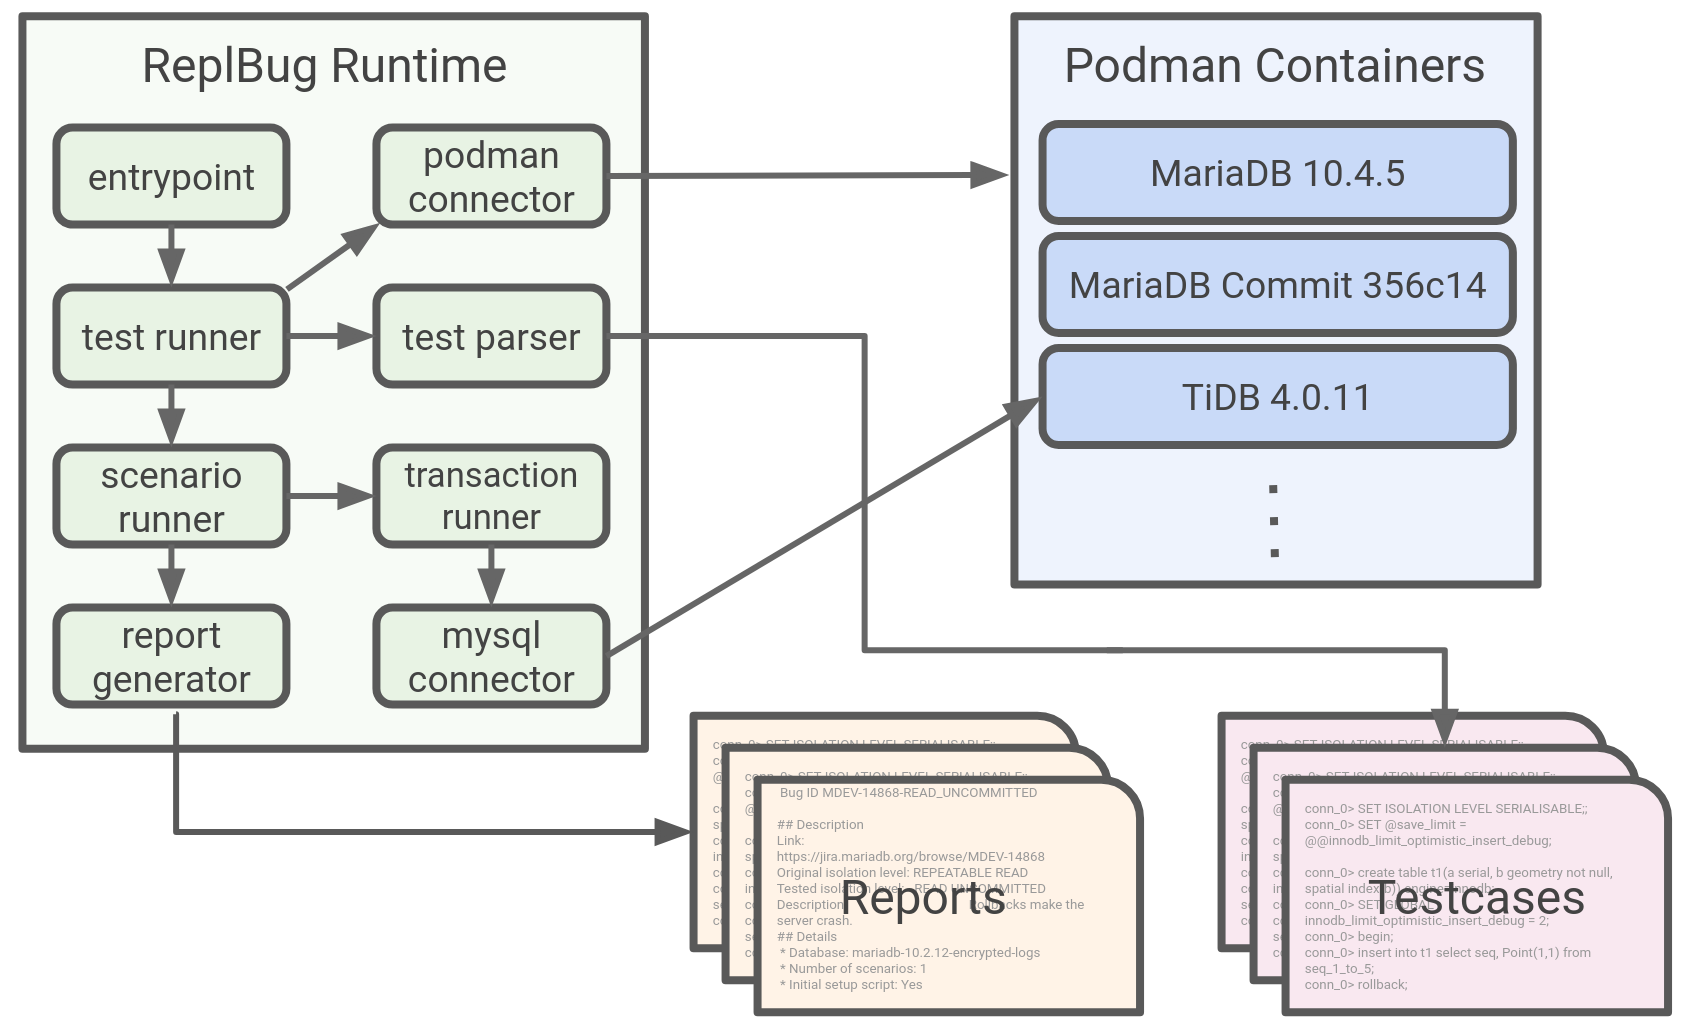
\includegraphics[width=\linewidth]{assets/replbug_design.png}
    \caption{Design of the \textit{ReplBug} testing framework}
    \label{fig:replb_design}
\end{figure}


The framework is modular, helping any future developer to easily extend it (for instance for adding support for new DBMSs). The main components in the bug testing pipeline (see Figure \ref{fig:replb_design}) are the following:

\begin{itemize}
    \item The \textit{podman connector}: This component handles the interaction with the \textit{Podman} engine, and is responsible for starting, stopping, downloading and managing containers running DBMS instances.
    \item The \textit{test parser}: This component handles the parsing of testcases, using a specific format, and is responsible for creating the internal representation of the testcases.
    \item The \textit{mysql connector}: This component handles the connection to a DBMS instance (running within a container), and is responsible for executing statements in order and extracting the results.
    \item The \textit{transaction runner}: This component handles the execution of all the statements in a transaction, and runs on different threads for concurrency.
    \item The \textit{scenario runner}: This component runs testcases under a specific configuration.
    \item The \textit{test runner}: This component orchestrates the execution of all required testcases under all specified configurations. 
\end{itemize}

\section{Custom DBMS Version}

Some bugs are specific to a certain version of a DBMS, which might not be available as pre-built binaries. For instance, versions with serious vulnerabilities are usually removed from official repositories, or intermediary versions tied to a specifig \textit{Git} commit are not released as binaries.

For the mentioned reasons, we consider the ability to built DBMSs from source essential. To simplify the process, we provide sample \textit{Dockerfile} templates, which can be used to test specific DMBS versions. A sample \textit{Dockerfile} for \textit{TiKV} can be seen in Figure \ref{fig:dockerfilesample}.
 
\begin{figure}
\begin{minted}[bgcolor=bg]{Dockerfile}
FROM golang:1.19-alpine AS builder

# Install git and other dependencies
RUN apk add --no-cache git make bash gcc wget binutils-gold \
    musl-dev curl tar

# Set the working directory inside the container and
# create necessary directories
RUN mkdir -p /go/src/github.com/pingcap
WORKDIR /go/src/github.com/pingcap

ARG TIDB_COMMIT=c9288d246c99073ff04304363dc7234d9caa5090

# Clone and build the TiDB repository
RUN git clone --depth 1 https://github.com/pingcap/tidb.git \
    && cd tidb \
    && git fetch --depth 1 origin "$TIDB_COMMIT" \
    && git checkout "$TIDB_COMMIT" \
    && make -j \
    && mv bin/tidb-server /usr/local/bin/tidb-server \
    && cd .. \
    && rm -rf tidb

EXPOSE 4000
WORKDIR /usr/local/bin
CMD ["./tidb-server", "-P", "4000"]    
\end{minted}
\caption{Sample \textit{Dockerfile} for building a specific version of \textit{TiDB}}
\label{fig:dockerfilesample}
\end{figure}

In our project, we provide \textit{Dockerfiles} for \textit{MySQL}, \textit{MariaDB} in release or debug mode, and \textit{TiDB} with or without \textit{TiKV}. Creating a new docker file only requires the \textit{Git} commit, and then running the \textit{build} command integrated into \textit{ReplBug}. 

\section{Testing Meta-Language}

For a given testcase, specifying the statements and their execution order on the DBMS is hard, due to multiple reasons:
\begin{itemize}
    \item Transactional and isolation bug PoCs usually need multiple concurent transactions, making a simple \textit{SQL} script insufficient.
    \item Some statements are expected to fail, which might lead to the termination of a standard script.
    \item The order of the statement execution (and sometimes the locking order) is important for the bug to manifest.
\end{itemize} 

To address these issues, the \textit{MySQL} development team created a testing framework which encodes testcases in a special format \cite{mysqltestrun}. Using this format, however, is cubersome, as we only need a small subset of the features, and using the \textit{MySQL} interpreter would make it hard to test other DBMSs. 

We thus create a small, custom scripting language on top of \textit{Python}, inspired by the way bug reporters describe their PoCs. In Figure \ref{fig:bug_metalanguage_sample}, we present a sample testcase for the bug \textit{MDEV-26642} in \textit{MariaDB 10.6.17}.

\begin{figure}
\begin{minted}[bgcolor=bg]{Python}
ORIGINAL_ISOLATION_LEVEL = DEFAULT_ISOLATION_LEVEL
BUG_ID = "MDEV-26642"
LINK = "https://jira.mariadb.org/browse/MDEV-26642"
DB_AND_VERSION = db_config.DatabaseTypeAndVersion(
    db_config.DatabaseType.MARIADB, "10.6.17"
)
SETUP_SQL_SCRIPT = """
create table t(a int, b int);
insert into t values (0, 0), (1, 1), (2, 2);
"""

DESCRIPTION = "The last select does not respect the update
                (a should always be 10)."


def get_scenarios(isolation_level: IsolationLevel):
    return [
        f"""
        conn_0> SET GLOBAL TRANSACTION ISOLATION LEVEL
                                {isolation_level.value};
        conn_0> begin;
        conn_0> select * from t;
        conn_1> begin;
        conn_1> update t set a = 10 where b = 1;
        conn_1> commit;
        conn_0> select * from t;
        conn_0> update t set a = 10 where true;
        conn_0> select * from t;
        conn_0> commit;
        """,
    ]
\end{minted}
\caption{Replication script for the bug \textit{MDEV-26642} in \textit{MariaDB 10.6.17}.} \label{fig:bug_metalanguage_sample}
\end{figure}

Each testcase provides the following information:
\begin{itemize}
    \item The \textit{DBMS} and version on which the bug was reported.
    \item The bug ID and a link to the bug report.
    \item The setup script, which is executed before the testcases. If the setup script is too long, it can be stored in a separate file.
    \item The description of the bug.
    \item The scenarios, which are the testcases that will be executed (one for each isolation level). Each scenario is a sequence of statements, executed in parallel by different connections.
\end{itemize}

For running a testcase, the tool provisions the required DBMS instance, executes the setup script (if present), and then runs the scenarios under all supported isolation levels. For each transaction a separate connection to the DBMS server is created. The results are then stored in a report, which can be further analysed.

\section{Usage}



\begin{figure}
    \centering
    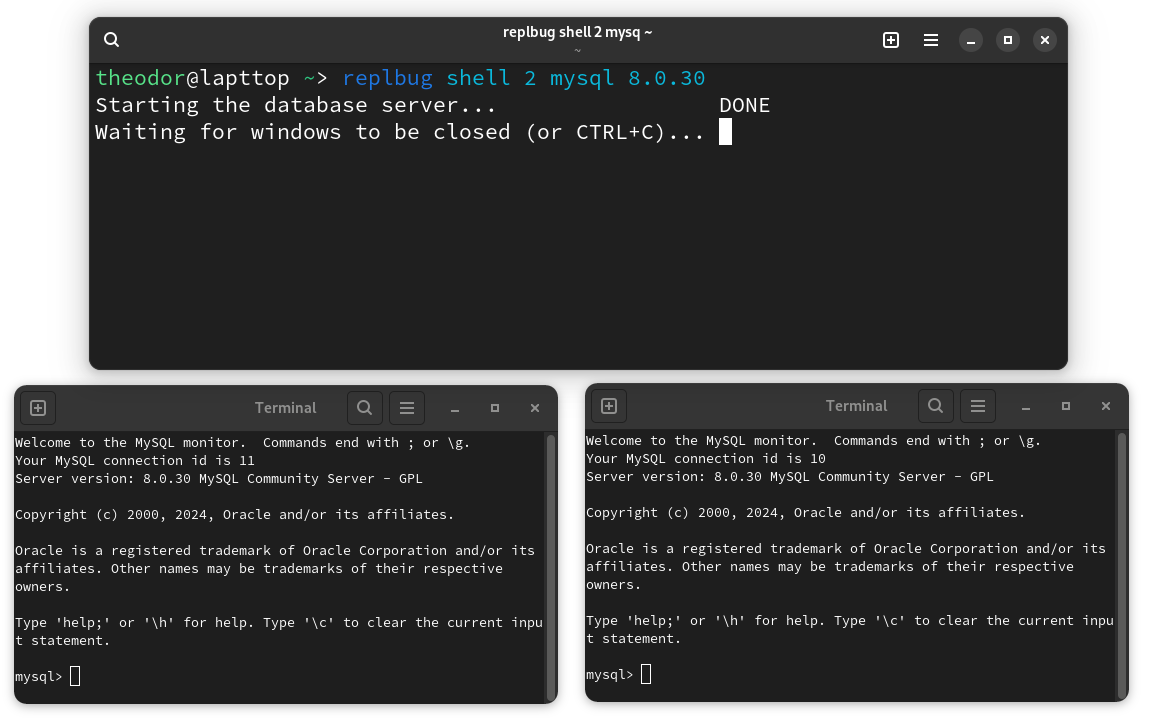
\includegraphics[width=\linewidth]{assets/replbug_shell.png}
    \caption{Using \textit{ReplBug} to start 2 \textit{MySQL v8.0.30} shells}
    \label{fig:replb_shell}
\end{figure}

\begin{figure}
    \centering
    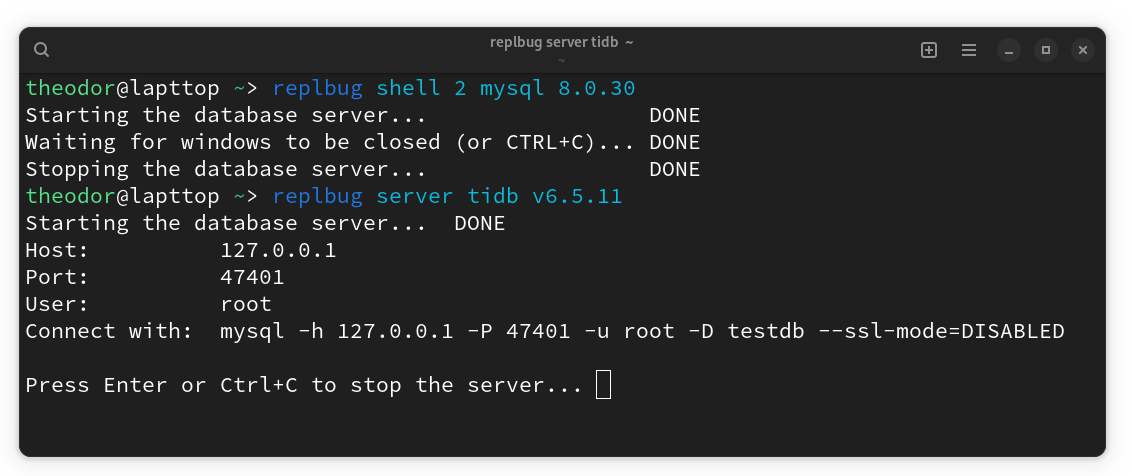
\includegraphics[width=\linewidth]{assets/replbug_server.png}
    \caption{Using \textit{ReplBug} to start a \textit{TiDB v6.5.11} server}
    \label{fig:repl_server}
\end{figure}

\begin{figure}
    \centering
    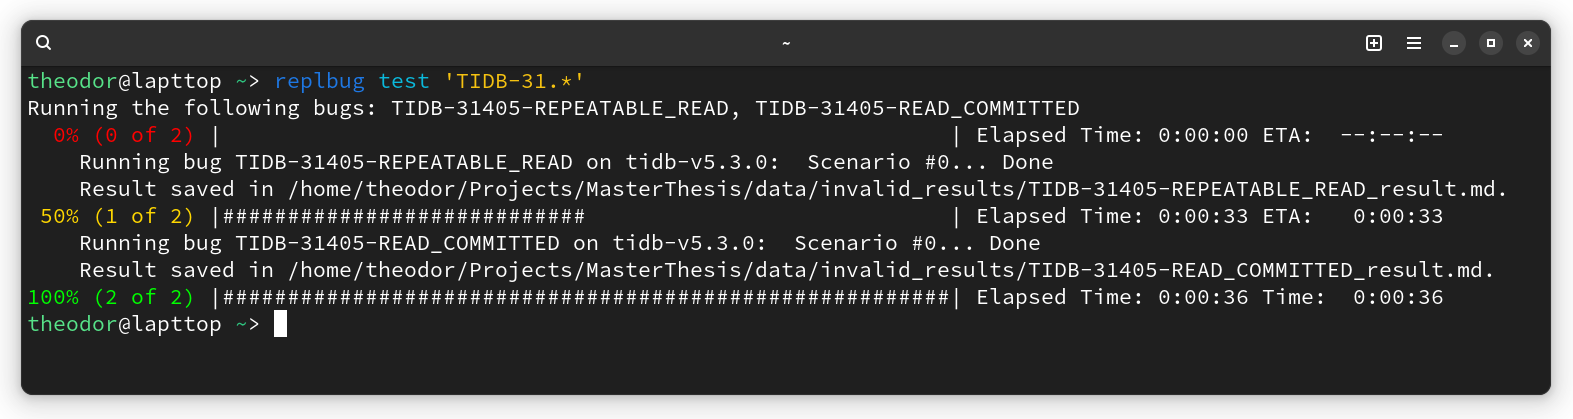
\includegraphics[width=\linewidth]{assets/replbug_test.png}
    \caption{Using \textit{ReplBug} to generate reports of some known bugs}
    \label{fig:repl_test}
\end{figure}


\begin{figure}
    \centering
    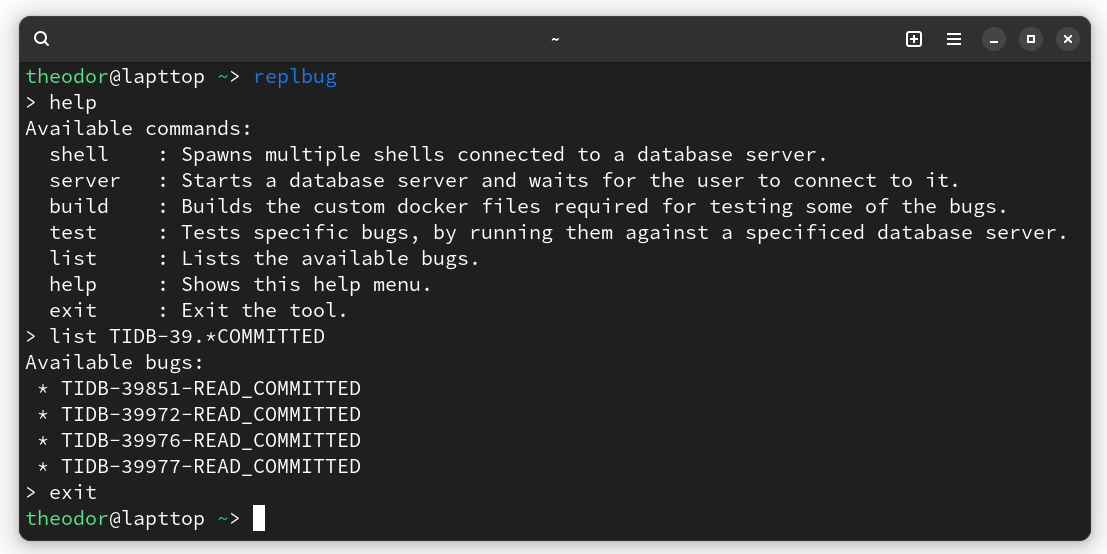
\includegraphics[width=\linewidth]{assets/replbug_interactive.png}
    \caption{Using \textit{ReplBug} in interactive mode}
    \label{fig:repl_interactive}
\end{figure}




The testing framework, called \textit{ReplBug} is invoked from the CLI. The main features it offers, exposed by the executable as subcommands are the following:
\begin{itemize}
    \item \textbf{\code{shell}} (See Figure \ref{fig:replb_shell}): Starts one or multiple \textit{MySQL}, \textit{MariaDB} or \textit{TiDB} shells, connected to a specific version of the DBMS. If the version is not present on the local machine, the tool will attempt to pull the image from Docker Hub.
    \item \textbf{\code{server}} (See Figure \ref{fig:repl_server}): Starts a specific version of the \textit{MySQL}, \textit{MariaDB} or \textit{TiDB} DBMS and provides the required details (host, port, user) for connecting to the server.
    \item \textbf{\code{test}} (See Figure \ref{fig:repl_test}): Runs the scenarios of some known bugs (which have to be written in a specific format prior), and automatically generates reports of the execution.
    \item \textbf{\code{list}}: Returns a list of the testcases available in the tool (optionally a \textit{regex} can be passed to filter the results).
\end{itemize}

The tool can be either used from the CLI by passing arguments, or in interactive mode, where the tool exposes a shell that can be used by the user  (see Figure \ref{fig:repl_interactive}).

\chapter{Replicating Transactional Bugs in MySQL, MariaDB and TiDB}

\section{Overview}

With the help of the \textit{ReplBug} testing framework, we were able to replicate \textit{MySQL}, \textit{MariaDB} and \textit{TiDB} transactional, logical and isolation bugs. We focus on transaction and isolation bugs, reported by DBMS testing papers \cite{cui2024understanding_ICSE2024, dou2023detecting_ICSE2023, cui2022differentially_ASE2022}. We then replicate the bugs on the same versions of the DBMSs, and verify which isolation levels are affected. The number of bugs taken from each paper can be seen in Figure \ref{fig:bugs_by_paper}.

\section{Replicated Bugs}


We try to replicate \textit{MySQL} and \textit{MariaDB} bugs on the $4$ isolation levels supported by the DBMSs (\textit{Read Uncommitted}, \textit{Read Committed}, \textit{Repeatable Read} and \textit{Serializable}). For \textit{TiDB}, we replicate the bugs on the $2$ isolation levels supported by the DBMS (\textit{Read Committed} and \textit{Serializable}).

\begin{figure}
    \centering
    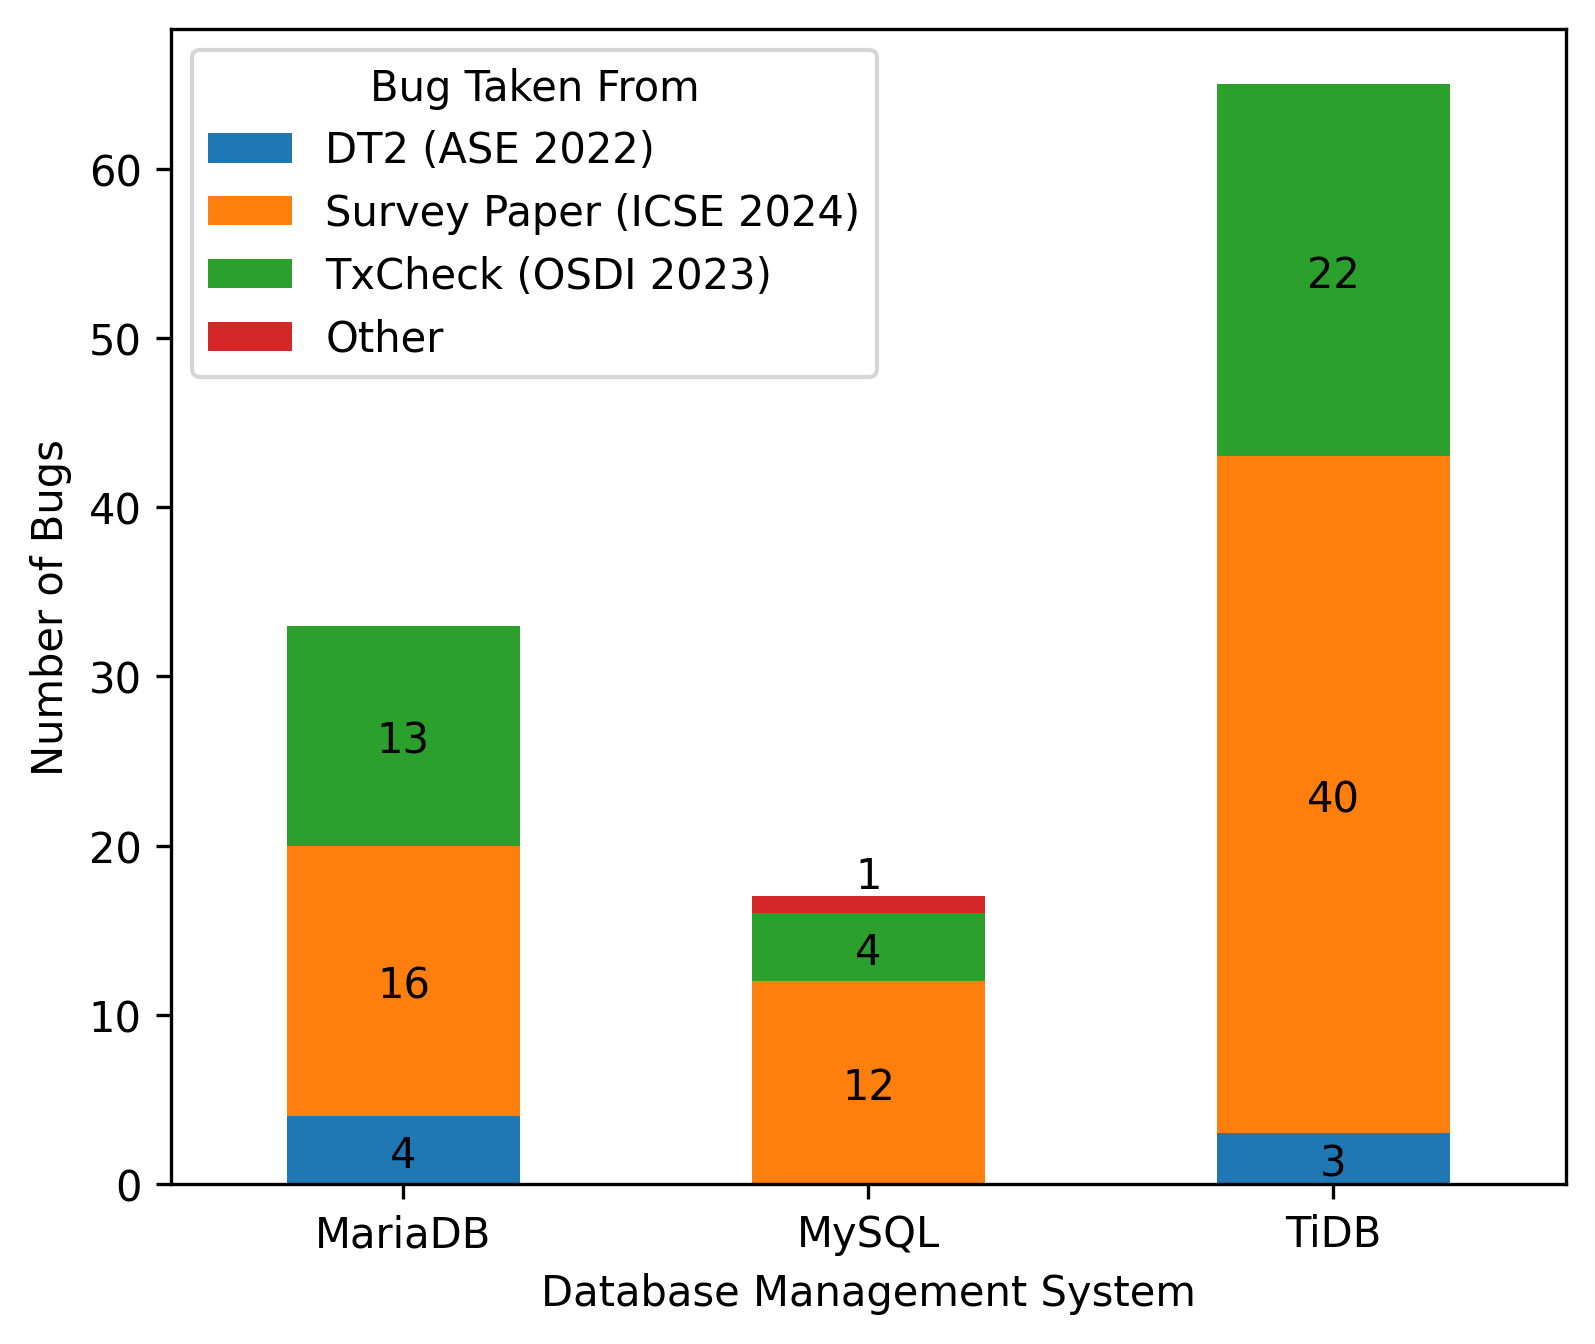
\includegraphics[width=0.8\linewidth]{assets/bug_replication_bugs_by_dbms_and_paper.png}
    \caption{Distribution of bugs by DBMS and reporting paper  \cite{cui2024understanding_ICSE2024, dou2023detecting_ICSE2023, cui2022differentially_ASE2022}.}
    \label{fig:bugs_by_paper}
\end{figure}

The methodology for replicating a bug is the following:
\begin{itemize}
    \item We search for the list of bugs reported by a paper, and filter the bugs that are transactional or isolation bugs (as reported by the paper), and manifest on one of the DBMSs we support (\textit{MySQL}, \textit{MariaDB} and \textit{TiDB}).
    \item We read the bug report in the DBMS's bug tracker, extract the version of the DBMS on which the bug was reported and a PoC.
    \item If the DBMS version is not available as a pre-built binary, we build the DBMS from source using the \textit{Dockerfile} templates provided by the \textit{ReplBug} tool.
    \item We write a testcase in the \textit{ReplBug} testing framework, using the meta-language described in the previous chapter.
    \item We run the testcase on the DBMS, under all supported isolation levels.
    \item We sometimes have to adjust the testcase, as some reports do not include the exact version of the DBMS, or the PoC is precise enough. 
\end{itemize}

Within this project, we successfully replicated $115$ bugs, out of which $33$ manifest on the \textit{MariaDB} DBMS, $17$ manifest on \textit{MySQL} and $65$ manifest on \textit{TiDB}. The distribution of the bugs by DBMS and reporting paper can be seen in Figure \ref{fig:interesting_bugs_by_paper}.

\section{Analysis}

We run the \textit{ReplBug} testing framework on the selected bugs, and we generate reports of their execution. We then read the reports, and analyse the output of the testcases. We then explore the corelation between the bugs and the isolation levels.

We find that $100$ bugs manifest on all isolation levels supported by the DBMS, and $15$ bugs only manifest on a subset of the isolation levels. In the reminder of this chapter, we refer to the bugs that manifest only on a subset of the isolation levels as \textit{interesting bugs}. In Figure \ref{fig:interesting_bugs_by_paper}, we present the distribution of the \textit{interesting bugs} by DBMS and reporting paper.

\begin{figure}
    \centering
    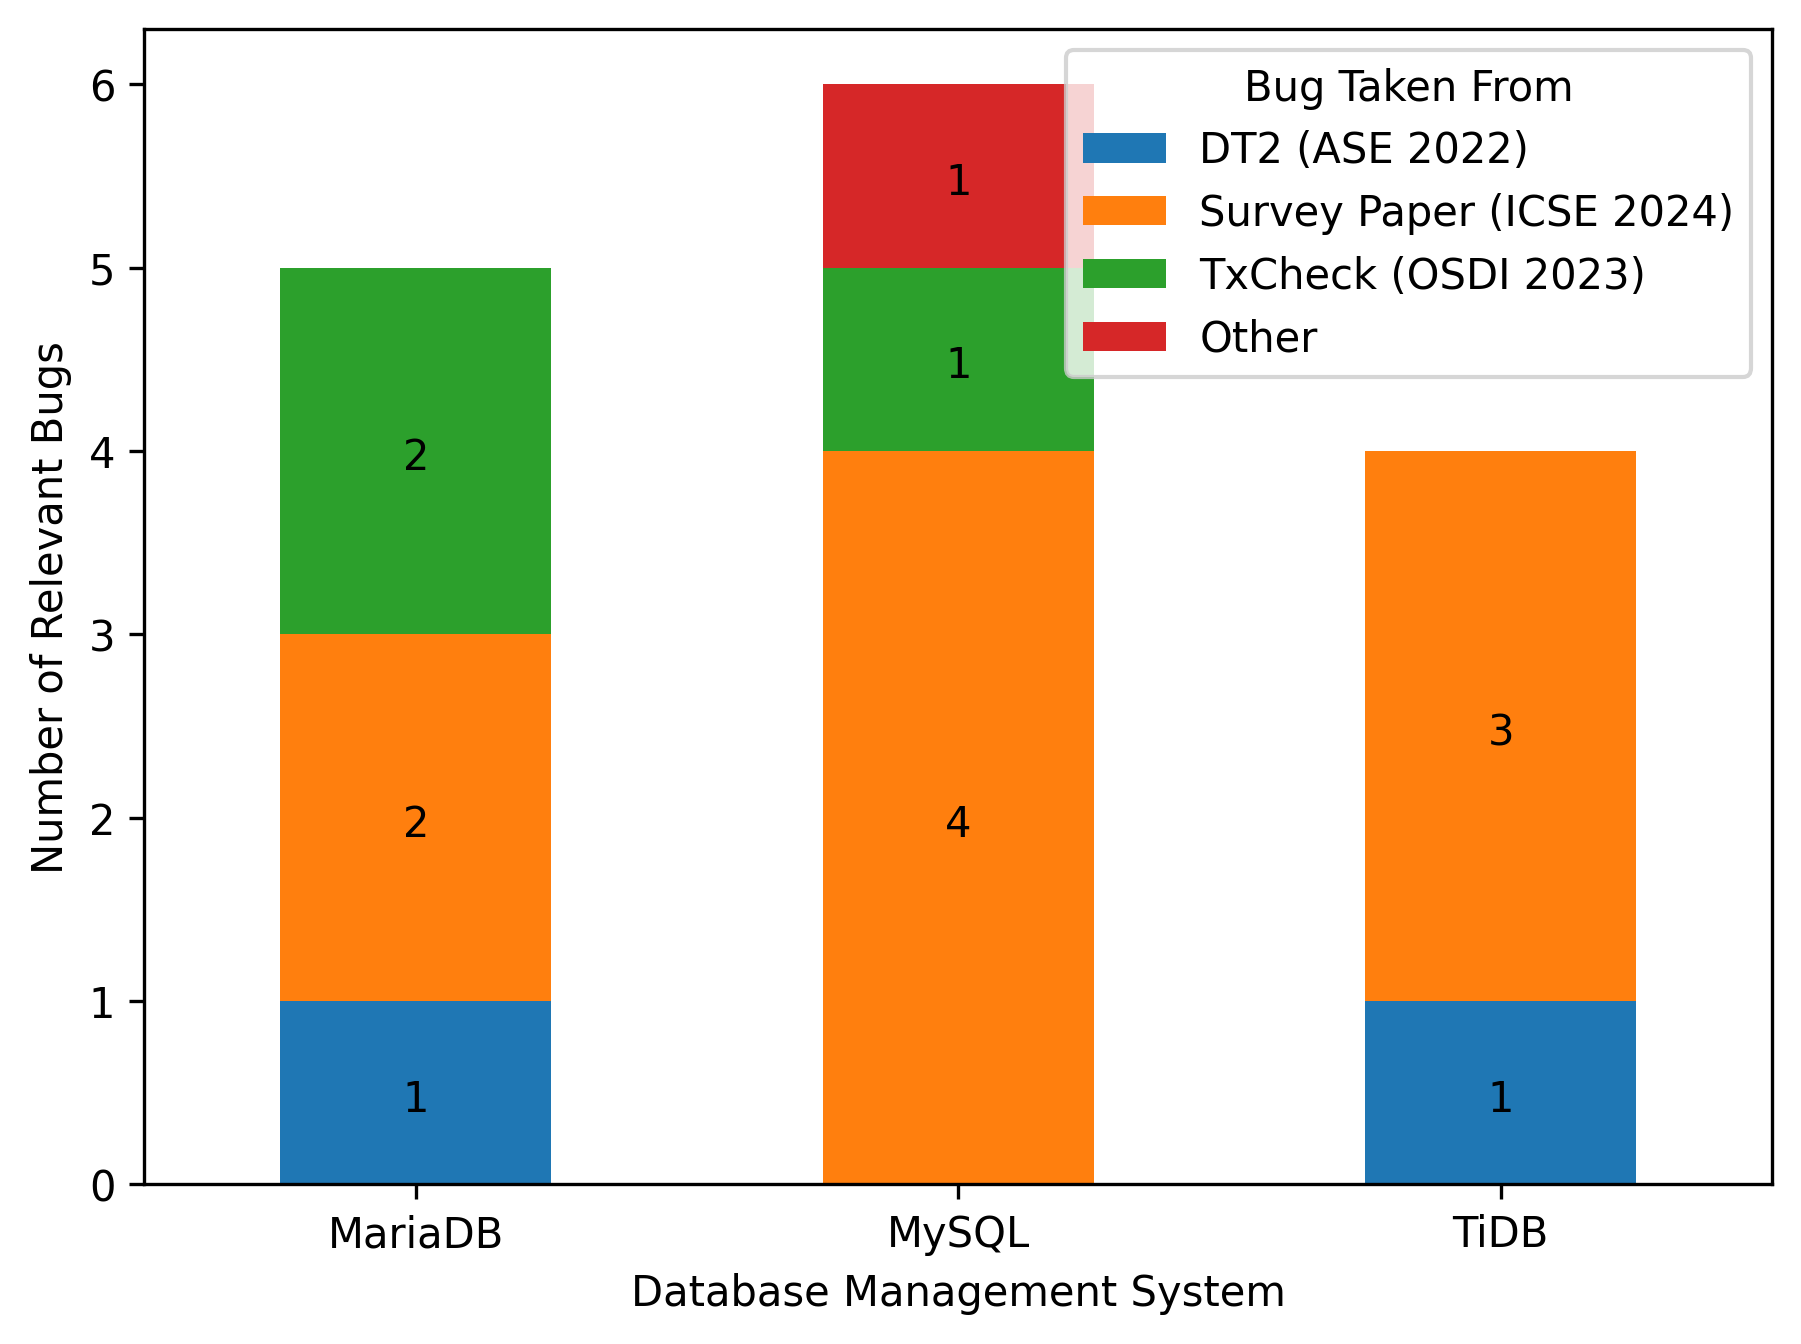
\includegraphics[width=0.8\linewidth]{assets/bug_replication_interesting_bugs_by_dbms_and_paper.png}
    \caption{Relevant bugs by DBMS and reporting paper  \cite{cui2024understanding_ICSE2024, dou2023detecting_ICSE2023, cui2022differentially_ASE2022}.}
    \label{fig:interesting_bugs_by_paper}
\end{figure}


We then explore the isolation levels under which the \textit{interesting bugs}, manifest. We find that:
\begin{itemize}
\item 5 bugs manifest under \textit{Read Committed} and \textit{Repeatable Read}.
\item 4 bugs manifest under \textit{Repeatable Read}.
\item 2 bugs manifest under \textit{Read Uncommitted} and \textit{Read Committed}.
\item 2 bugs manifest under \textit{Read Committed}.
\item One bug manifests under \textit{Serializable}.
\item One bug manifests under \textit{Repeatable Read} and \textit{Serializable}.
\end{itemize}

The findings are illustrated in Figure \ref{fig:interesting_bugs_by_isolation_lvl}. The main limitation of this analysis is that the number of \textit{intersting bugs} is small, making the results not statistically significant. Additionally, our approach only allows us to verify if a bug is triggered by a specific PoC, and not to explore the root cause of the bug, which could in theory be triggered by other PoCs under different isolation levels.

\begin{figure}
    \centering
    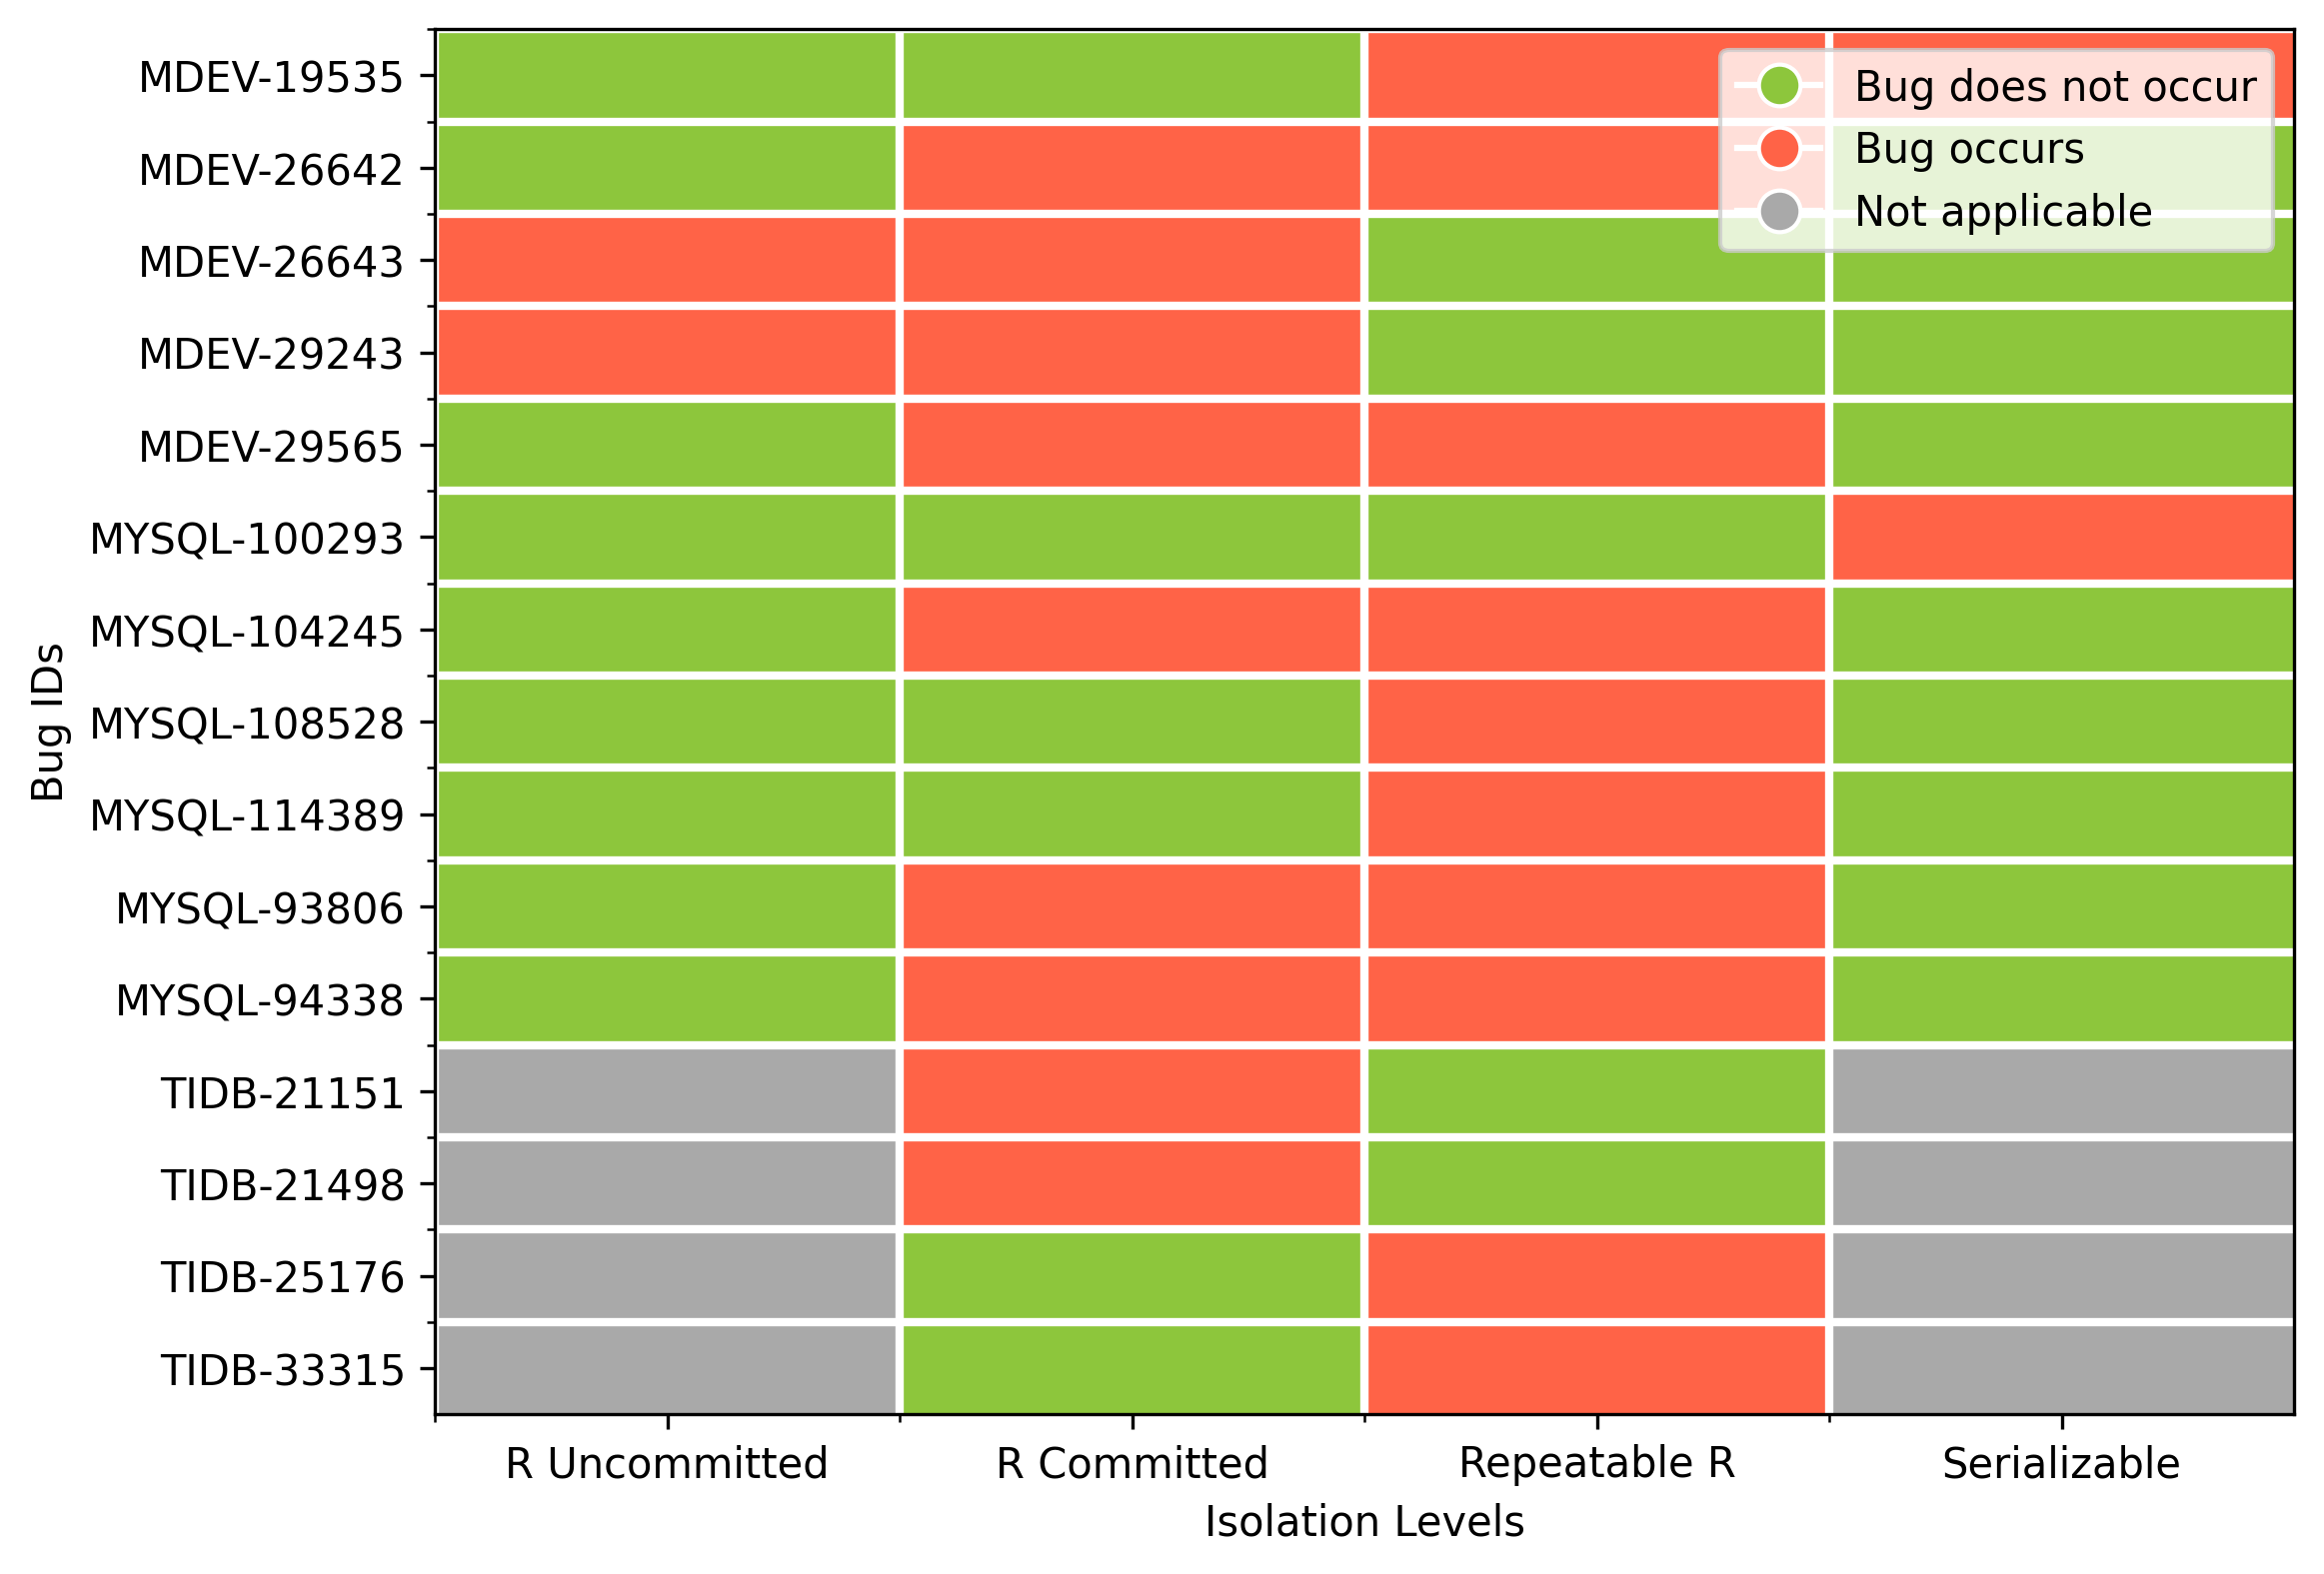
\includegraphics[width=0.9\linewidth]{assets/bug_replication_interesting_bugs_by_isolation_lvl.png}
    \caption{Relevant bugs by isolation levels.}
    \label{fig:interesting_bugs_by_isolation_lvl}
\end{figure}

\section{Interesting Bugs}

We present a brief overview of the \textit{interesting bugs}, and provide a plausible explanation for their behaviour, where possible. The bugs are presented in the order of the number of isolation levels under which they manifest.

\subsection*{Bug MDEV-19535}

This bug is replicated on \textit{MariaDB 10.4.5}, and manifests under \textit{Repeatable Read} and {Serializable}.

For compatibility, \textit{MariaDB} provides an \code{sql\_mode} variable, which can be used to mimic the behaviour of other DBMSs.

When the \code{sql\_mode} is set to \code{ORACLE}, \textit{MariaDB} ommits to add exclusive locks when running an \textit{SELECT FOR UPDATE} statement. This leads to incorrect hehaviour when running \textit{SELECT FOR UPDATE} statements under \textit{Repeatable Read} and \textit{Serializable} isolation levels, as reads are no longer guaranteed to be repeatable.

\subsection*{Bug MDEV-26642}


This bug is replicated on \textit{MariaDB 10.6.17}, and manifests under \textit{Read Committed} and \textit{Repeatable Read}. The bug was fixed by a PR in version \textit{$10.6.18$}, and was marked as affecting \textit{MySQL} too.


The bug affects concurent modifications of the same table: if a transaction updates a row of the table, and another transaction updates the entire table, the second transaction does not see its own modifications. The main part of the PoC can be seen in Figure \ref{fig:MDEV-26642}.


\begin{figure}
\begin{minted}[bgcolor=bg]{SQL}
conn_0> begin;
conn_0> select * from t;        -- [(0, 0), (1, 1), (2, 2)]

conn_1> begin;
conn_1> update t set a = 10 where b = 1;
conn_1> commit;

conn_0> select * from t;        -- [(0, 0), (1, 1), (2, 2)]
conn_0> update t set a = 10 where true;
conn_0> select * from t;        -- [(10, 0), (1, 1), (10, 2)]
conn_0> commit;
\end{minted}
\caption{PoC for the bug \textit{MDEV-26642}.} \label{fig:MDEV-26642}
\end{figure}

The bug is caused by a design issue of \textit{InnoDB}, the storage engine used by both \textit{MariaDB} and \textit{MySQL}.

The bug is due to the inability of \textit{InnoDB} to detect \textit{write-write} conflicts. Under \textit{Read Committed} and \textit{Repeatable Read}, \textit{InnoDB} creates a read view at the start of a statement / transaction, used for knowing which records should be visible, but does not handle overwriten records properly. 

The \textit{Read Uncommitted} isolation level always displays the latest state of the table, and \textit{Serializable} will lock the accessed records first, so the bug does not manifest under these isolation levels.

\subsection*{Bug MDEV-26643}


This bug is replicated on \textit{MariaDB 10.5.12}, and manifests under \textit{Read Uncommitted} and \textit{Read Committed}. The bug was fixed by a PR.The PoC is very similar to \textit{MDEV-26642}, and can be seen in Figure \ref{fig:MDEV-26643}.


\begin{figure}
\begin{minted}[bgcolor=bg]{SQL}
conn_0> insert into t values(null, 1), (2, 2),
                    (null, null), (null, 3), (4, null);
conn_0> begin;
conn_0> update t set a = 10 where 1;
conn_1> begin;
conn_1> update t set b = 20 where a;
conn_0> commit;
conn_1> commit;
conn_2> select * from t; 
        -- [(10, 1), (10, 20), (10, 20), (10, 20), (10, 20)]
\end{minted}
\caption{PoC for the bug \textit{MDEV-26642}.} \label{fig:MDEV-26643}
\end{figure}

The bug is caused by an improperly used semi-consistent read, where \textit{Read Uncommitted} and \textit{Read Committed} transactions are sometimes not updated with the latest changes.

\subsection*{Bug MDEV-29243}

This bug is replicated on \textit{MariaDB 10.8.3}, and manifests under \textit{Read Uncommitted} and \textit{Read Committed}, by causing a crash of the DBMS server.

The root cause of the bug is an incorrect and redundant check of the data retrival status in \textit{InnoDB}, which leads to potential assertion failures. The bug was fixed by erasing the redundant check.

\subsection*{Bug MDEV-29565}

This bug is replicated on \textit{MariaDB 10.8.3}, and manifests under \textit{Read Committed} and \textit{Repeatable Read}.

While confirmed as intented behaviour, this is caused by an poorly documented feature of \textit{InnoDB}, which allows changes made by other transactions to be visible in the current one if changes are made to the same records \cite{mysqlconsistentread}. The PoC is simplified in Figure \ref{fig:MDEV-29565}.

\begin{figure}
\begin{minted}[bgcolor=bg]{SQL}
conn_1> START TRANSACTION;
conn_1> update t set a = 162;
conn_0> START TRANSACTION;
conn_1> COMMIT;
conn_0> select * from t where <CONDITION>; -- returns 1 record
conn_0> update t set a = 63 where <CONDITION>;
conn_0> select * from t where a = 63;      -- returns 2 records
conn_0> COMMIT;
\end{minted}
\caption{Simplification of the PoC for the bug \textit{MDEV-29565}.} \label{fig:MDEV-29565}
\end{figure}


\subsection*{Bug MYSQL-100293}

This bug is replicated on \textit{MySQL 5.7.31}, and manifests under \textit{Serializable}.

When the \code{innobase\_query\_caching\_of\_table\_permitted} flag is set to \code{true} (by passing \code{--query-cache-type=1} as an argument to the server), \textit{Serialisable} transactions are not blocked when using the cache, which causes some missing locks.

The bug was fixed by properly handling \code{--query-cache-type=1} when the transaction isolation level is \textit{Serializable}.

\subsection*{Bug MYSQL-104245}


This bug is replicated on \textit{MySQL 8.0.23}, and manifests under \textit{Read Committed} and \textit{Repeatable Read}.

Wen inserting rows with the same primary key multiple times (using the \code{INSERT IGNORE} statement), row locks are duplicated. Using \code{REPLACE INTO} is even worse, and adds many row locks (we believe the number of added locks is the number of matched records times the number of inserted records).

The bug only manifests on \textit{Read Committed} and \textit{Repeatable Read}, as \textit{Serializable} has a different locking mechanism, and \textit{Read Uncommitted} does not lock the records at all.

This bug dramatically increases latency, but does not cause deadlocks or crashes, as all the redundant row locks are identical. The bug is not present in \textit{MySQL 8.0} or later, so it was not fixed.

\subsection*{Bug MYSQL-108528}

This bug is replicated on \textit{MySQL 5.7.34}, and manifests under \textit{Repeatable Read}.

The bug is marked as verified, but we strongly consider the PoC actually works as intented. The PoC is simplified in Figure \ref{fig:MYSQL-108528}.

In the PoC, one transaction updates a table and commits. Another concurent transaction does not see the changes made by the first transaction, however those changes become visible when the second transaction tried to update a table. This behaviour is similar to the behaviour of \textit{MDEV-29565}, and we consider it is due to the same poorly-documented feature \cite{mysqlconsistentread}.


\begin{figure}
\begin{minted}[bgcolor=bg]{SQL}
    conn_1> START TRANSACTION;
    conn_0> START TRANSACTION;
    conn_0> select * from t_rpjlsd;         -- Create snapshot.

    conn_1> update t_g6ckkb set wkey = 162; -- Update the table.
    conn_1> COMMIT;                         -- Commit.

    conn_0> select * from t_rpjlsd where
                t_rpjlsd.c_pfd8ab <= (
                    select min(wkey)
                    from t_g6ckkb
                );                          -- Affects 1 row.
    conn_0> update t_rpjlsd set wkey = 63 where
                t_rpjlsd.c_pfd8ab <= (
                    select min(wkey)
                    from t_g6ckkb
                );                          -- Affects 2 rows.
\end{minted}
\caption{Simplification of the PoC for the bug \textit{MYSQL-108528}.} \label{fig:MYSQL-108528}
\end{figure}



\subsection*{Bug MYSQL-114389}

This bug is replicated on \textit{MySQL 8.0.12}, and manifests under \textit{Repeatable Read}. The bug is still present in the latest version of \textit{MySQL} (version \textit{9.1.0}). It was closed as \textit{duplicate}, but the original bug is still open.

As the bug is still open, we do not know the root cause of the bug, whose PoC can be seen in Figure \ref{fig:MYSQL-114389}.

\begin{figure}
\begin{minted}[bgcolor=bg]{SQL}
conn_0> BEGIN;

conn_1> BEGIN;                          
conn_1> UPDATE t SET b = 222, c = 333;   -- Update the table.
conn_1> COMMIT;                         

conn_2> BEGIN;
conn_2> SELECT pkId, b, c FROM t;        -- Create snapshot.

conn_0> UPDATE t SET a = 40 WHERE a = 44;
conn_0> COMMIT;

conn_2> UPDATE t SET b = 888, c = 999;   -- Update the table.
conn_2> SELECT pkId, b, c FROM t where   -- Should be empty but
          b = 854 or c = 333 order by b; -- returns a row.

\end{minted}
\caption{PoC for the bug \textit{MYSQL-114389}.} \label{fig:MYSQL-114389}
\end{figure}


\subsection*{Bug MYSQL-93806}

This bug is replicated on \textit{MySQL 8.0.12}, and manifests under \textit{Read Committed} and \textit{Repeatable Read}. The bug was fixed as part of the \textit{MySQL 8.0.16} release.

The bug is caused by a misshandling of the \code{INSERT ... ON DUPLICATE KEY} statement. When a record with a conflicting primary key is inserted, the key should be changed and a row lock created. However, under \textit{Read Committed} and \textit{Repeatable Read}, a range lock is created instead. The PoC is simplified in Figure \ref{fig:MYSQL-93806}.

\begin{figure}
\begin{minted}[bgcolor=bg]{SQL}
conn_0> create table t(id int primary key, a int)engine=innodb;
conn_0> insert into t values(1,1),(5,5);

conn_0> SET GLOBAL TRANSACTION ISOLATION LEVEL REPEATBLE READ;
conn_0> begin;
conn_0> insert into t values(5,5) ON DUPLICATE
            KEY UPDATE a=a+1; -- Creates a range lock instead
                              -- of a row lock.

conn_1> begin;
conn_1> insert into t values(4, 4); -- Is needlessly blocked by
                                    -- the range lock.
\end{minted}
\caption{Simplification of the PoC for the bug \textit{MYSQL-93806}.} \label{fig:MYSQL-93806}
\end{figure}


\subsection*{Bug MYSQL-94338}

This bug is replicated on \textit{MySQL 5.7.25}, and manifests under \textit{Read Committed} and \textit{Repeatable Read}. The bug is not present in \textit{MySQL 8.0} or later, so it was not fixed.

The bug manifests by causing diry-reads when inserting multiple rows on one transaction, and performing a complex query on another transaction. The PoC is simplified in Figure \ref{fig:MYSQL-94338}. We do not know the root cause of the bug, as no bug fix was made available.

\begin{figure}
\begin{minted}[bgcolor=bg]{SQL}

        conn_0> BEGIN;
        conn_1> BEGIN;

        conn_1> INSERT INTO t VALUES
                (1,40,'B',10,1),
                (1,41,'B',10,1),
                ...
                (1,40,'C',16,1),
                (1,42,'C',16,1);

        conn_0> SELECT * FROM t1
                WHERE <<CON`DITION>>; -- Dirty read.;
\end{minted}
\caption{Simplification of the PoC for the bug \textit{MYSQL-94338}.} \label{fig:MYSQL-94338}
\end{figure}

\subsection*{Bug TIDB-21151}

This bug is replicated on \textit{TiDB v4.0.8} when using the \textit{TiKV} key-value store, and manifests under \textit{Read Committed}. The bug was closed by a PR pushed to the \code{master} branch on \textit{2020-11-24}.

The bug occurs because the \code{USE\_INDEX\_MERGE} feature does not refresh the current timestamp of the transaction, causing the transaction to potentially miss the latest committed writes. While this is correct to \textit{REPETABLE READ} transactions, \textit{READ COMMITTED} transactions are expected to see committed changes. A simplified PoC can be seen in Figure \ref{fig:TIDB-21151}. 

The bug fix correctly updates the timestamp used by transactions when running under \textit{READ COMMITTED}, by invoking the \code{refreshForUpdateTSForRC} function when required.

\begin{figure}
\begin{minted}[bgcolor=bg]{SQL}
conn_0> BEGIN;

-- Update the table, after transaction 0 started.
conn_1> BEGIN;
conn_1> update t set value = 11 where id = 2;
conn_1> COMMIT;

conn_0> select /*+ NO_INDEX_MERGE() */ *
            from t where a > 3 or b > 3;   -- Ok.

conn_0> select /*+ USE_INDEX_MERGE(t, ia, ib) */ *
            from t where a > 3 or b > 3;   -- Misses the update.
\end{minted}
\caption{Simplification of the PoC for the bug \textit{TIDB-21151}.} \label{fig:TIDB-21151}
\end{figure}

\subsection*{Bug TIDB-21498}

This bug is replicated on \textit{TiDB}, on the custom commit \code{3a32bd2d} using the \textit{TiKV} key-value store, and manifests under \textit{Read Committed}. The bug was closed by a PR pushed to the \code{master} branch on \textit{2021-01-12}.

The bug occurs because of missing consistency checks which allow one concurent transaction to perform DDL (Data Definition Language) operations on a table (like inserting / deleting columns or deleting indexes), while another transaction is reading from the same table. The PoC is simplified in Figure \ref{fig:TIDB-21498}.

\begin{figure}
\begin{minted}[bgcolor=bg]{SQL}
conn_0> begin;

conn_1> alter table t drop index iv;
conn_1> update t set v = 11 where id = 1;

conn_0> select * from t where v = 10; -- Returns [1, 10].
conn_0> select * from t where id = 1; -- Returns [1, 11].
\end{minted}
\caption{Simplification of the PoC for the bug \textit{TIDB-21498}.} \label{fig:TIDB-21498}
\end{figure}

\subsection*{Bug TIDB-25176}

This bug was reported on a specific commit of the \code{master} branch, is replicated on \textit{TiDB 4.0.7} when using the \textit{TiKV} key-value store, and manifests under \textit{Repeatable Read}. The bug is still open as of \textit{November 2024}.

The bug is due to the usage of the \code{tidb\_snapshot} system variable, which sets the timestamp delimiting the visibility of the records \cite{tidbsnapshot}. 

Under \textit{Repetable Read}, setting this timestamp and the performing a \code{SELECT} statement breaks the isolation level guarantees. The PoC is simplified in Figure \ref{fig:TIDB-25176}.

\begin{figure}
\begin{minted}[bgcolor=bg]{SQL}
conn_0> begin;                              -- Start txn.
    
conn_1> update test.ttt set a=2 where id=1; -- Update records.

conn_0> set @@tidb_snapshot=TIMESTAMP(NOW());

conn_0> select a from test.ttt where id=1;            -- [(1)].
conn_0> select a from test.ttt where id=1 for update; -- [(2)].
conn_0> select a from test.ttt where id=1;            -- [(2)].
\end{minted}
\caption{Simplification of the PoC for the bug \textit{TIDB-25176}.} \label{fig:TIDB-25176}
\end{figure}

\subsection*{Bug TIDB-33315}

This bug is replicated on \textit{TiDB 5.4.0} when using the \textit{TiKV} key-value store, and manifests under \textit{Repeatable Read}. 

The bug is caused by the mismatch of rows created by concurent transactions: if a transaction performs a statement matching an entire table while another transaction holds an exclusive lock on the table, the first transaction will see an inconsistent state. The PoC is simplified in Figure \ref{fig:TIDB-33315}.

\begin{figure}
\begin{minted}[bgcolor=bg]{SQL}
conn_0> BEGIN PESSIMISTIC;
conn_0> UPDATE t SET c1=2, c2=2;

conn_1> BEGIN PESSIMISTIC;
conn_1> DELETE FROM t;     -- Delete all records.

conn_0> COMMIT;            -- First transaction commits.

conn_1> SELECT * FROM t;   -- Returns one row.
conn_1> COMMIT;
\end{minted}
\caption{Simplification of the PoC for the bug \textit{TIDB-33315}.} \label{fig:TIDB-33315}
\end{figure}


\section{Conclusion}

In this chapter, we present an analysis of a few isolation bugs we consider \textit{interesting}, as they manifest under a subset of the isolation levels supported by the DBMSs. We provide a brief overview of the bugs, and a plausible explanation for their behaviour.

We find that the bugs are caused by a variety of reasons, from design issues of the storage engine to poorly documented features of the DBMSs. We also find that some bugs are quickly fixed, while others are left unfixed until they \textit{fix themselves}, i.e. they are no longer present in the latest versions of the DBMSs.

The main cause of bugs is the improper handling of locking and MVCC (Multi-Version Concurrency Control) mechanisms, which are the core of the transactional guarantees provided by the DBMSs, as \textit{MySQL}, \textit{MariaDB} and \textit{TiDB} define their isolation levels based on locking behaviour and transaction visibility \cite{mysqlisolationlevels,mariadbtransactions,tidbisolationlevels}.

% \chapter{Practical Snapshot Isolation}
% \section{Natural Concurrency Control}
\section{Practical Snapshot Isolation}


\subsection{Key Observations and Motivations}
In this project, we are targeting distributed systems that 
are used for web applications. 
First, \cite{lu2023ncc} makes some key observations about transactions in web applications.

\begin{enumerate}
    \item Transactions in web applications are usually short. This means that the possibility that transactions interleave with each other and induce write-write or read-write conflict is small.
    \item Transactions in web applications are usually read-dominant. This means interleaving read requests  is fine.
    \item In usual network environments, transactions will arrive naturally in the order they submit.
\end{enumerate}

By combining the observations, we can conclude that most transactions in web applications will naturally satisfy the snapshot isolation level.  However, existing snapshot isolation protocols take a pessimistic view of transaction conflicts. They use excessive locks, extra rounds of messages, etc. to ensure that transactions satisfy the snapshot isolation level even if they satisfy that naturally. Instead, we take a practical view of snapshot isolation. We have already observed that most transactions in web applications naturally satisfy snapshot isolations. We abort those transactions that do not satisfy snapshot isolation properties or violate committed transactions' read visibility. Our design is heavily inspired by \cite{lu2023ncc}.


\subsection{Overall Architecture}
\begin{figure}[H]
    \centering
    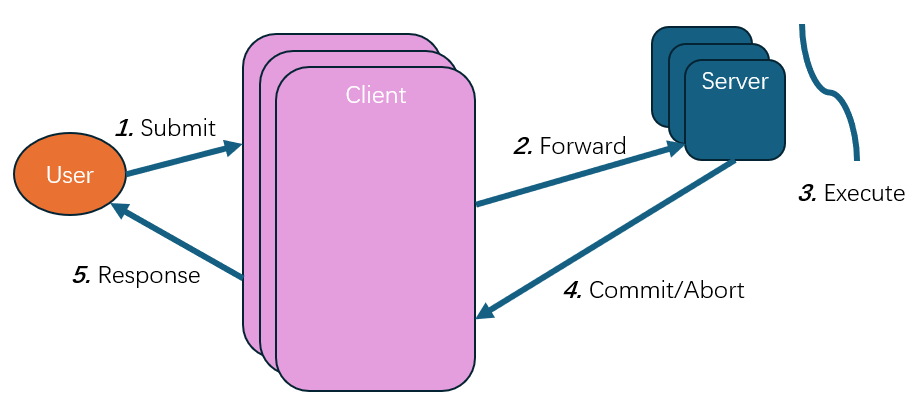
\includegraphics[width=0.8\linewidth]{figure/overall.png}
    \caption{Overall Architecture of Our Proposed Methods}
    \label{fig:overall}
\end{figure}

Figure \ref{fig:overall} describes our proposed methods' architecture. There are many clients and servers for scalability reasons. Each server holds one partition of the data. In the first step, users submit a transaction request to a client. In the second step, the client will look at the requests inside the transaction and forward the request to the server based on the request content (such as the hash value of the key involved in the transaction). The client will also assign a timestamp (such as a physical clock) to the transaction. In the third step, the server that receives the request will execute them in a non-blocking fashion, as we assume that most transactions will naturally satisfy the snapshot isolation property. After the execution finishes, the server will check whether the transaction satisfies the snapshot isolation properties. In rare cases where this transaction violates some properties, the server simply aborts it. In the fourth step, the server will send the decision on the commit/abort and the result to the client. In the fifth step, the client will return the result to the user.
\subsection{Non-blocking Execution}

The server will maintain the latest version tag for each data item it stores. 
The server executes the requests in a non-blocking manner. This means the server executes requests just as in a single thread. Moreover, when a read request is received, the server will execute the request and associate the result with its latest version. When a write request is received, the server will create a new version associated with that data item and associate that version with this write operation. This non-blocking execution greatly enhances the performance because it does not require blocking operations such as locking, extra rounds of messages.


\subsection{Server Side Algorithms}
Here we present our algorithms used at the server side. We adapt \cite{lu2023ncc} for snapshot isolation.


\begin{algorithm}
\caption{Server-side Algorithm for Executing Transactions of Practical Snapshot Isolation}
\label{alg:cap}
\begin{algorithmic}
\Require $S$ is a multi-version data store. $S[version][key]$ will retrieve the data item with key $key$ at the version $version$.
\Require $T$ is the transaction to be executed.
\Require $t$ is the latest system (or snapshot) version.
\Require $f(key)$ will return the largest version
of data item $key$ that is smaller than $t$. 
\Require $\mathcal{R}$ is the return result set.
\State $t^\prime \gets$  $t$ \Comment{Remember the system version before the transaction $T$}

\For{$r \in T$} \Comment{First, we execute all the requests in a non-blocking fashion.}
    \State $\mathcal{R}[r.key] \gets S[f(t^\prime)][r.key]$     \Comment{Retrieve the latest version result.}

\If {$r$ is a write request}
   % \State $\mathcal{R}[r.key] \gets S[t^\prime][r.key]$
    \State $t^\prime \gets t^\prime + 1$
    \State $S[t^\prime][r.key] \gets r.value$

\EndIf
\EndFor
\State $commit \gets true$
\Comment {Next, we will check whether to commit this transaction or not}
\For{$r \in T$}
\If {$r$ is a read request}
    \If {$t^\prime > f(r.key)$} \Comment{Read a future value, abort!}
    \State $commit \gets false$
    \EndIf
\Else \Comment{$r$ is a write request}
    \If {$t^\prime < f(r.key)$} \Comment{Overwrite a commit value, abort!}
    \State $commit \gets false$
    \EndIf
\EndIf
\EndFor


% \While{Server Does Not Receive a Request}
% \EndWhile
% \State $y \gets 1$
% \State $X \gets x$
% \State $N \gets n$
% \While{$N \neq 0$}
% \If{$N$ is even}
%     \State $X \gets X \times X$
%     \State $N \gets \frac{N}{2}$  
%     \Comment{This is a comment}
% \ElsIf{$N$ is odd}
%     \State $y \gets y \times X$
%     \State $N \gets N - 1$
% \EndIf
% \EndWhile
\end{algorithmic}
\end{algorithm}





\begin{algorithm}
\caption{The commit algorithm}\label{alg:commit}
\begin{algorithmic}
\Require $commit$ is $true$.
\Require $T$ the transaction to be executed
\State $t \gets t^\prime$ \Comment{Update the system version.}
\For {$r \in T$} \Comment{Update $f(key)$}
\If {$r$ is a write request}
\State $f(r.key) \gets t$
\EndIf
\EndFor
\end{algorithmic}
\end{algorithm}



\begin{algorithm}
\caption{The abort algorithm}\label{alg:abort}
\begin{algorithmic}
\Require $commit$ is $false$.
\Require $T$ the transaction to be aborted
\For {$r \in T$} 
% \Comment{Update $f(key)$}
\If {$r$ is a write request}
\State $S[f(r.key)][r.key] \gets \mathcal R[f(r.key)]$ \Comment{Rollback to the previous version}
\EndIf
\EndFor
\end{algorithmic}
\end{algorithm}


Algorithm \ref{alg:cap} is the main algorithm. Algorithm \ref{alg:commit} is the commit algorithm, and Algorithm \ref{alg:abort} is the abort algorithm. 
We use $S$ to record a multi-version data store, $t$ to record the latest system version, and $f(key)$ to retrieve the latest version of data item $key$. The algorithm first executes all requests in a non-blocking fashion. Then, it will check all requests and see if there are any read-write conflicts or write-write conflicts. If no such conflicts exist and the transaction can safely be committed, we update $t$ and $f(key)$ according to the commit algorithm. Otherwise, according to the abort algorithm, we will roll back $S$ to the previous version.  


\section{Experiments}
\subsection{Overview}
In this section, we will describe our experiments to demonstrate the performance of our practical snapshot isolation algorithm. We implemented three baselines. The first baseline we implemented is Clock-SI \cite{du2013clock}, a snapshot isolation algorithm that does not depend on a centralized clock. The second snapshot isolation algorithm we implemented is Percolator \cite{peng2010large}. Google widely uses the Percolator system to process incremental updates to a large data set. The Percolator system supports snapshot isolation protocol and provides an industrial common standard for implementing distributed snapshot isolation concurrency control levels. The third baseline we implemented is Walter \cite{sovran2011transactional}. It also supports (parallel) snapshot isolation. We will first introduce the three baselines. Then, we will introduce the experiment setup. Next, we will introduce and analyze the results of the experiment. Finally,  we will conclude this chapter. 


% \subsection{Clock-SI}



% \subsection{Percolator}
% \subsection{Walter}
\subsection{Experimental Setup}

\paragraph{Code Base.} We used the same code base as \cite{lu2023ncc} for implementing our practical snapshot isolation algorithms. We also used the same code base for implementing Clock-SI \cite{du2013clock}, Percolator \cite{peng2010large}, Walter \cite{sovran2011transactional}.

\paragraph{Workloads.} We used the YCSB benchmark \cite{cooper2010benchmarking}. YCSB is a key-value benchmark that Yahoo collects for many usages, including testing the performance of key-value stores, different concurrency control protocols. We mainly used workload A for testing. Workload A is a read-dominant workload, but the read-write ratio could be tuned for different purposes. Unless otherwise stated, we use the default parameter settings in YCSB.

\paragraph{Setup.} We used the CloudLab \cite{duplyakin2019design} as the testbed.  We used the XL170 node on the Utah cluster. The machine has 2 10-Core, 3.4 GHz, Xeon E5-2640 v4 CPUs and the network bandwidth is 10Gbps. 




\subsection{Results for Different Read Ratios}
We experiment with our methods with three other baselines under different read ratios. Refer to Figure \ref{fig:31}, Figure \ref{fig:32}, Figure \ref{fig:33}. Results show that our method outperforms three other baselines under different read ratio.

\begin{figure}[H]
    \centering
    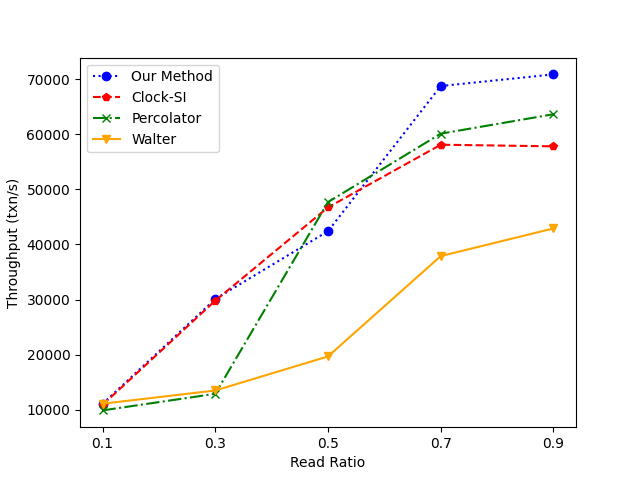
\includegraphics[width=0.8\linewidth]{figure/31.png}
    \caption{Throughput Comparison for Different Concurrency Control Algorithms for Different Read Ratio}
    \label{fig:31}
\end{figure}
\begin{figure}[H]
    \centering
    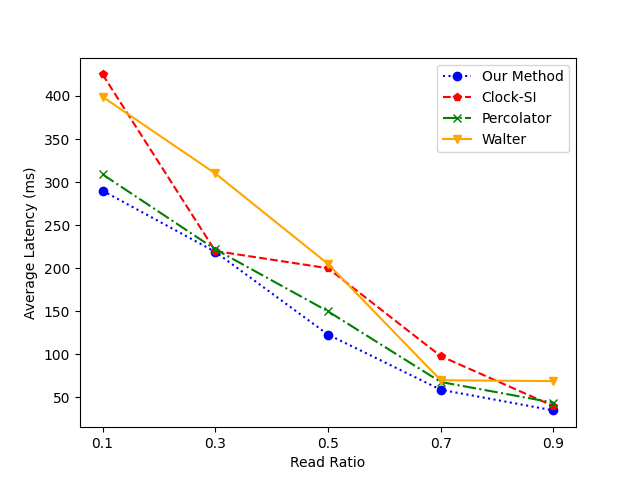
\includegraphics[width=0.8\linewidth]{figure/32.png}
    \caption{Average Latency for Different Concurrency Control Algorithms for Different Read Ratio}
    \label{fig:32}
\end{figure}
\begin{figure}[H]
    \centering
    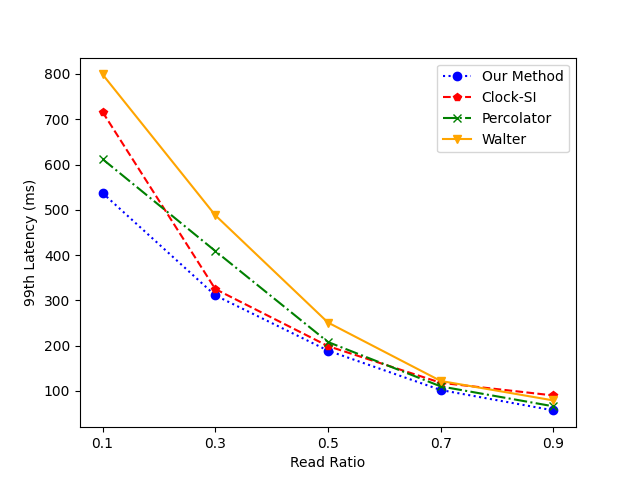
\includegraphics[width=0.8\linewidth]{figure/33.png}
    \caption{99th Latency for Different Concurrency Control Algorithms for Different Read Ratio}
    \label{fig:33}
\end{figure}



\subsection{Results for Different Transaction Sizes}
We experiment with our methods with three other baselines under different transaction sizes. Refer to Figure \ref{fig:34}, Figure \ref{fig:35}, Figure \ref{fig:36}. Results show that our method outperforms three other baselines under different transaction size.

\begin{figure}[H]
    \centering
    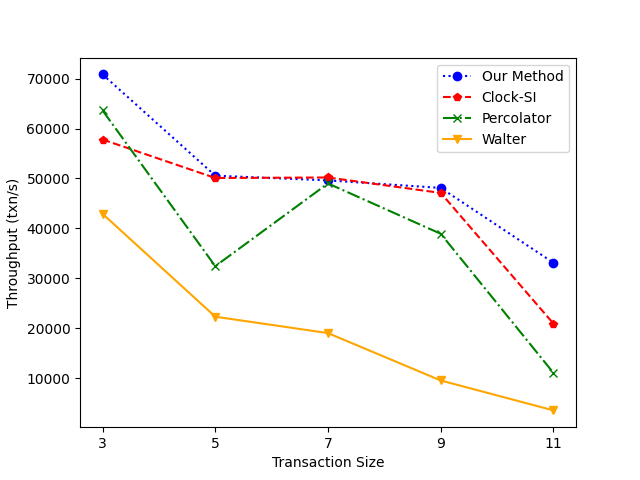
\includegraphics[width=0.8\linewidth]{figure/34.png}
    \caption{Throughput Comparison for Different Concurrency Control Algorithms for Different Transaction Size}
    \label{fig:34}
\end{figure}
\begin{figure}[H]
    \centering
    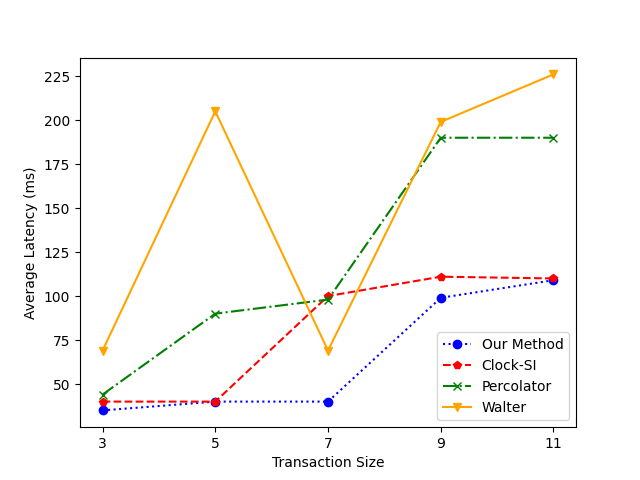
\includegraphics[width=0.8\linewidth]{figure/35.png}
    \caption{Average Latency for Different Concurrency Control Algorithms for Different Transaction Size}
    \label{fig:35}
\end{figure}
\begin{figure}[H]
    \centering
    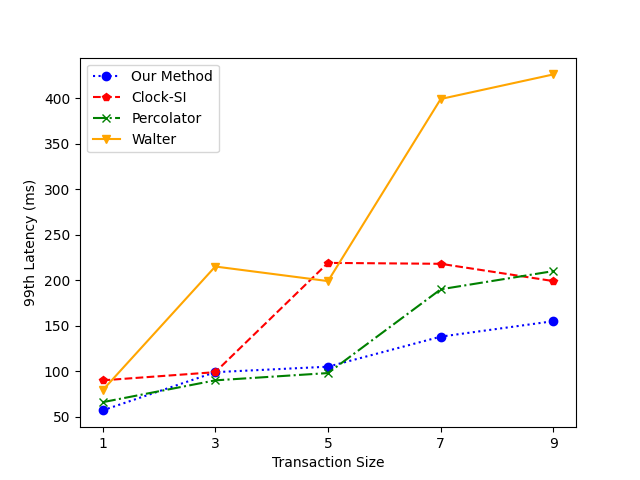
\includegraphics[width=0.8\linewidth]{figure/36.png}
    \caption{99th Latency for Different Concurrency Control Algorithms for Different Transaction Size}
    \label{fig:36}
\end{figure}








\subsection{Results for Different Numbers of Servers}

We experiment with our methods with three other baselines under different number of servers. Refer to Figure \ref{fig:37}, Figure \ref{fig:38}, Figure \ref{fig:39}. Results show that our method outperforms three other baselines under different number of servers.

\begin{figure}[H]
    \centering
    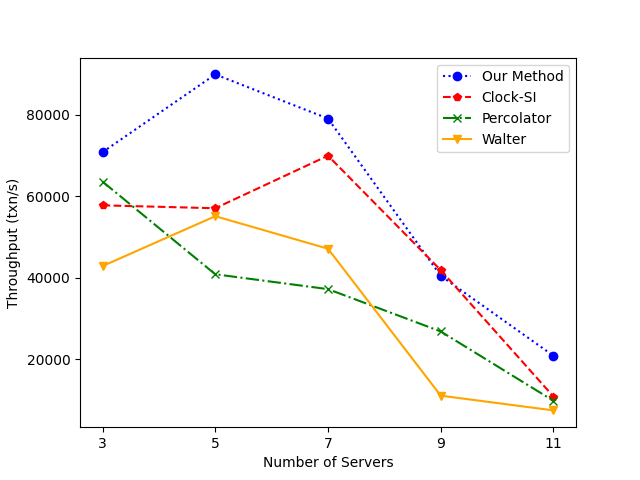
\includegraphics[width=0.8\linewidth]{figure/37.png}
    \caption{Throughput Comparison for Different Concurrency Control Algorithms for Different Number of Servers}
    \label{fig:37}
\end{figure}
\begin{figure}[H]
    \centering
    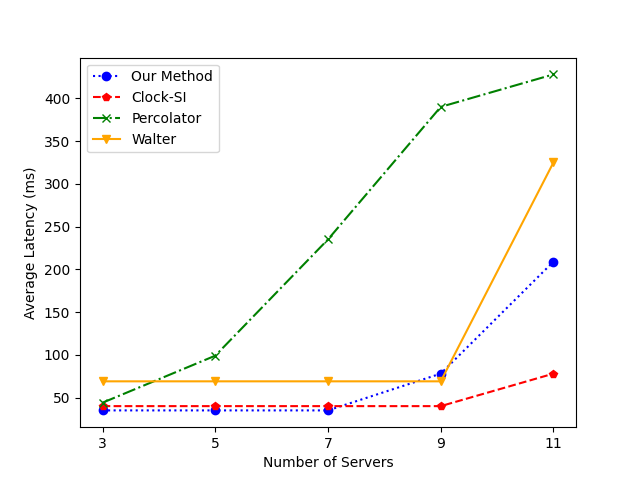
\includegraphics[width=0.8\linewidth]{figure/38.png}
    \caption{Average Latency for Different Concurrency Control Algorithms for Different Number of Servers}
    \label{fig:38}
\end{figure}
\begin{figure}[H]
    \centering
    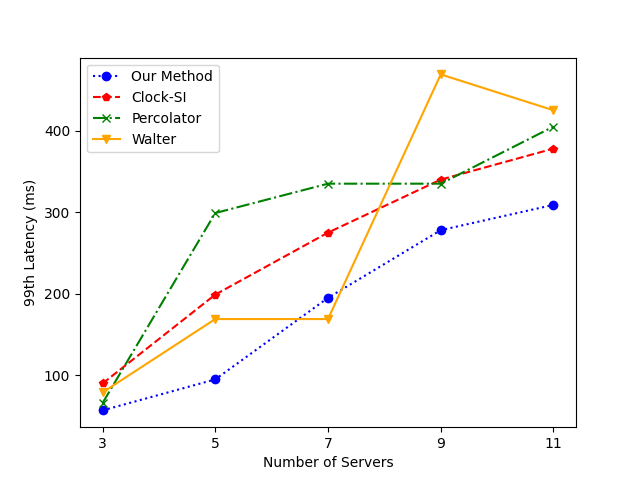
\includegraphics[width=0.8\linewidth]{figure/39.png}
    \caption{99th Latency for Different Concurrency Control Algorithms for Different Number of Servers}
    \label{fig:39}
\end{figure}



\subsection{Results for Different Numbers of Clients}
We experiment with our methods with three other baselines under different number of clients. Refer to Figure \ref{fig:40}, Figure \ref{fig:41}, Figure \ref{fig:42}. Results show that our method outperforms three other baselines under different number of clients.

\begin{figure}[H]
    \centering
    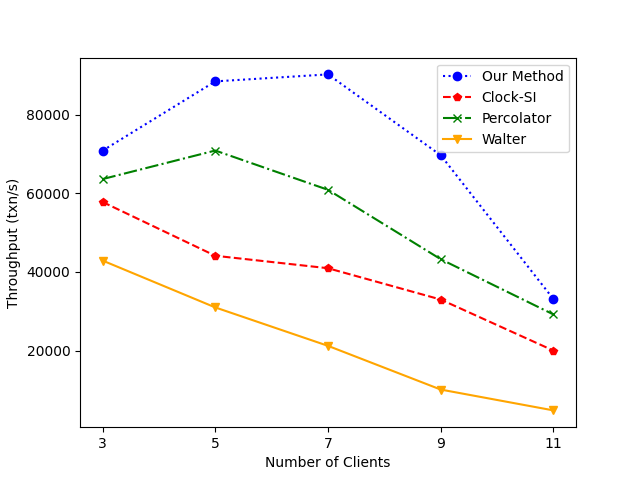
\includegraphics[width=0.8\linewidth]{figure/40.png}
    \caption{Throughput Comparison for Different Concurrency Control Algorithms for Different Number of Clients}
    \label{fig:40}
\end{figure}
\begin{figure}[H]
    \centering
    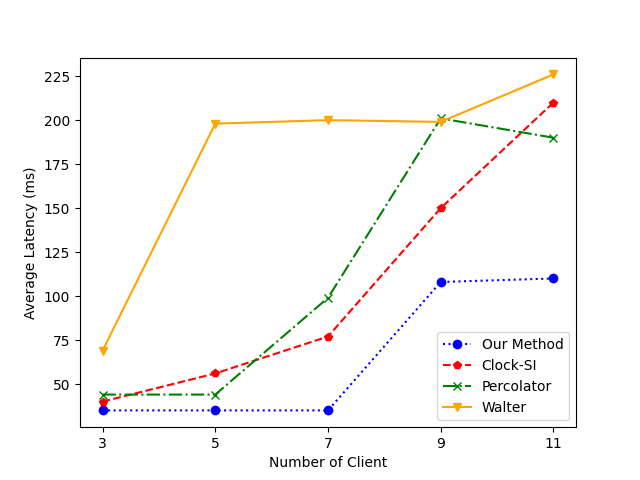
\includegraphics[width=0.8\linewidth]{figure/41.png}
    \caption{Average Latency for Different Concurrency Control Algorithms for Different Number of Client}
    \label{fig:41}
\end{figure}
\begin{figure}[H]
    \centering
    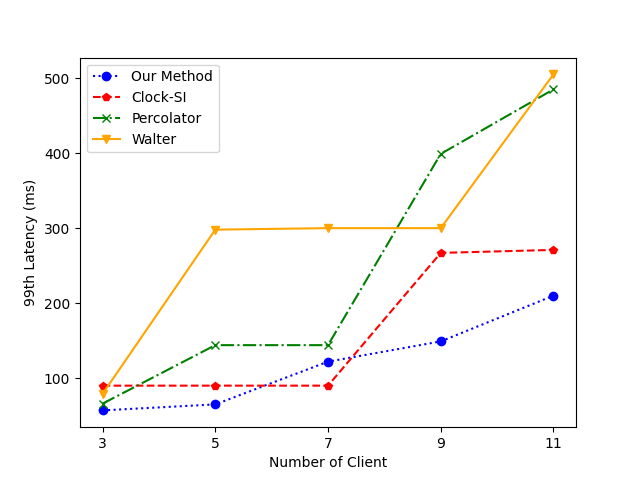
\includegraphics[width=0.8\linewidth]{figure/42.png}
    \caption{99th Latency for Different Concurrency Control Algorithms for Different Number of Clients}
    \label{fig:42}
\end{figure}



\subsection{Results for Different Value Sizes}
We experiment with our methods with three other baselines under different value size. Refer to Figure \ref{fig:43}, Figure \ref{fig:44}, Figure \ref{fig:45}. Results show that our method outperforms three other baselines under different value size.

\begin{figure}[H]
    \centering
    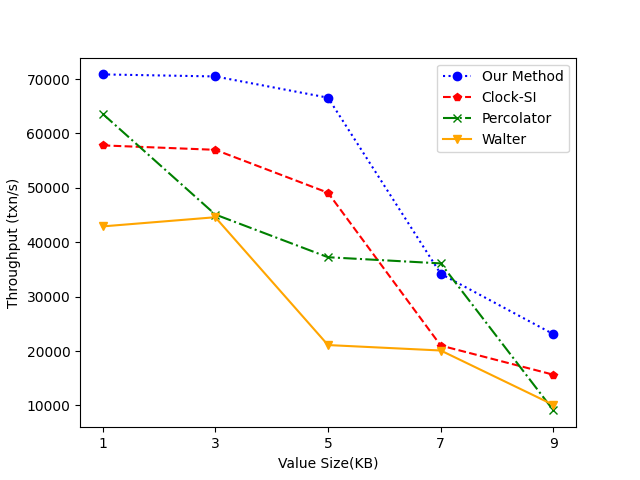
\includegraphics[width=0.8\linewidth]{figure/43.png}
    \caption{Throughput Comparison for Different Concurrency Control Algorithms for Different Value Size}
    \label{fig:43}
\end{figure}
\begin{figure}[H]
    \centering
    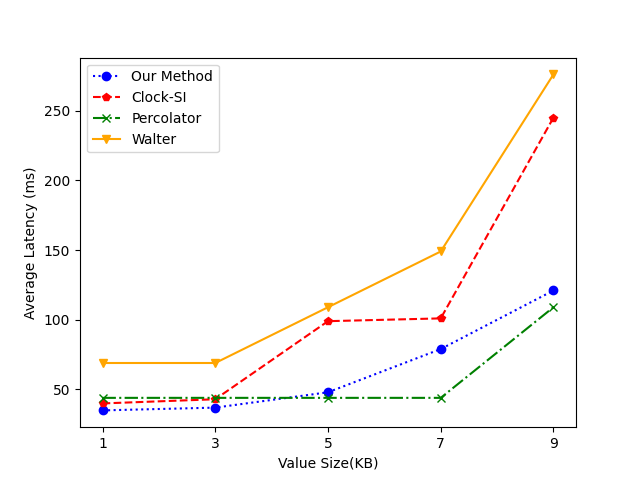
\includegraphics[width=0.8\linewidth]{figure/44.png}
    \caption{Average Latency for Different Concurrency Control Algorithms for Different Value Size}
    \label{fig:44}
\end{figure}
\begin{figure}[H]
    \centering
    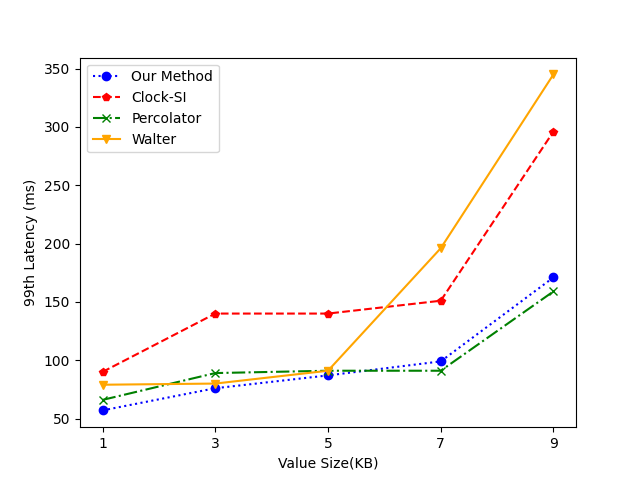
\includegraphics[width=0.8\linewidth]{figure/45.png}
    \caption{99th Latency for Different Concurrency Control Algorithms for Different Value Size}
    \label{fig:45}
\end{figure}




\subsection{Results for Different Numbers of Keys}

We experiment with our methods with three other baselines under different number of keys. Refer to Figure \ref{fig:46}, Figure \ref{fig:47}, Figure \ref{fig:48}. Results show that our method outperforms three other baselines under different number of keys.

\begin{figure}[H]
    \centering
    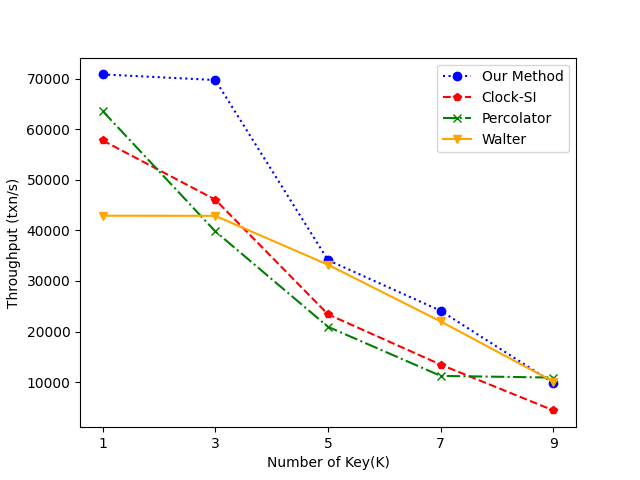
\includegraphics[width=0.8\linewidth]{figure/46.png}
    \caption{Throughput Comparison for Different Concurrency Control Algorithms for Different Number of Keys}
    \label{fig:46}
\end{figure}
\begin{figure}[H]
    \centering
    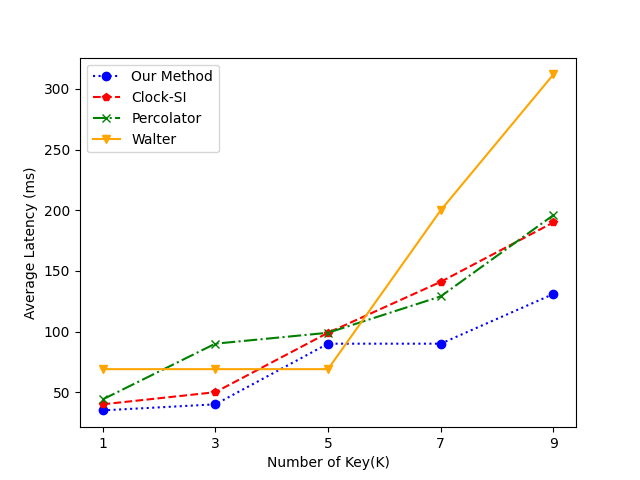
\includegraphics[width=0.8\linewidth]{figure/47.png}
    \caption{Average Latency for Different Concurrency Control Algorithms for Different Number of Keys}
    \label{fig:47}
\end{figure}
\begin{figure}[H]
    \centering
    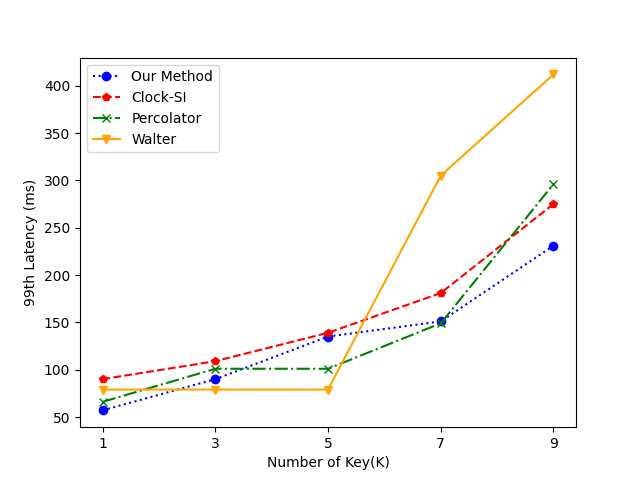
\includegraphics[width=0.8\linewidth]{figure/48.png}
    \caption{99th Latency for Different Concurrency Control Algorithms for Different Number of Keys}
    \label{fig:48}
\end{figure}




\subsection{Conclusions}
In this chapter, we have presented practical snapshot isolation algorithms based on the observation that most transactions will naturally be preserved in the order they submit by \cite{lu2023ncc}. As such, we take an optimistic approach. We execute the transaction without relying on external events such as lock. When the transaction is being committed, we will check whether the transaction satisfies the snapshot isolation properties. Our algorithms show  performance improvement over the three baselines implemented.

% \input{Conclusions}
% \chapter{Writing scientific texts in English}

This chapter was originally a separate document written by Reto
Spöhel.  It is reprinted here so that the template can serve as a
quick guide to thesis writing, and to provide some more example
material to give you a feeling for good typesetting.

% We're going to need an extra theorem-like environment for this
% chapter
\theoremstyle{plain}
\theoremsymbol{}
\newtheorem{Rule}[theorem]{Rule}

\section{Basic writing rules}

The following rules need little further explanation; they are best
understood by looking at the example in the booklet by Knuth et al.,
§2--§3.

\begin{Rule}
  Write texts, not chains of formulas.
\end{Rule}

More specifically, write full sentences that are logically
interconnected by phrases like `Therefore', `However', `On the other
hand', etc.\ where appropriate.

\begin{Rule}
  Displayed formulas should be embedded in your text and punctuated
  with it.
\end{Rule}

In other words, your writing should not be divided into `text parts'
and `formula parts'; instead the formulas should be tied together by
your prose such that there is a natural flow to your writing.

\section{Being nice to the reader}

Try to write your text in such a way that a reader enjoys reading
it. That's of course a lofty goal, but nevertheless one you should
aspire to!

\begin{Rule}
  Be nice to the reader.
\end{Rule}

Give some intuition or easy example for definitions and theorems which
might be hard to digest. Remind the reader of notations you introduced
many pages ago -- chances are he has forgotten them. Illustrate your
writing with diagrams and pictures where this helps the reader. Etc.

\begin{Rule}
  Organize your writing.
\end{Rule}

Think carefully about how you subdivide your thesis into chapters,
sections, and possibly subsections.  Give overviews at the beginning
of your thesis and of each chapter, so the reader knows what to
expect. In proofs, outline the main ideas before going into technical
details. Give the reader the opportunity to `catch up with you' by
summing up your findings periodically.

\emph{Useful phrases:} `So far we have shown that \ldots', `It remains
to show that \ldots', `Recall that we want to prove inequality (7), as
this will allow us to deduce that \ldots', `Thus we can conclude that
\ldots. Next, we would like to find out whether \ldots', etc.

\begin{Rule}
  Don't say the same thing twice without telling the reader that you
  are saying it twice.
\end{Rule}

Repetition of key ideas is important and helpful. However, if you
present the same idea, definition or observation twice (in the same or
different words) without telling the reader, he will be looking for
something new where there is nothing new.

\emph{Useful phrases:} `Recall that [we have seen in Chapter 5 that]
\ldots', `As argued before / in the proof of Lemma 3, \ldots', `As
mentioned in the introduction, \ldots', `In other words, \ldots', etc.

\begin{Rule}
  Don't make statements that you will justify later without telling
  the reader that you will justify them later.
\end{Rule}

This rule also applies when the justification is coming right in the
next sentence!  The reasoning should be clear: if you violate it, the
reader will lose valuable time trying to figure out on his own what
you were going to explain to him anyway.

\emph{Useful phrases:} `Next we argue that \ldots', `As we shall see,
\ldots', `We will see in the next section that \ldots, etc.


\section{A few important grammar rules}

\begin{Rule}
  \label{rule:no-comma-before-that}
  There is (almost) \emph{never} a comma before `that'.
\end{Rule}

It's really that simple. Examples:
\begin{quote}
  We assume that \ldots\\
  \emph{Wir nehmen an, dass \ldots}

  It follows that \ldots\\
  \emph{Daraus folgt, dass \ldots}

  `thrice' is a word that is seldom used.\\
  \emph{`thrice' ist ein Wort, das selten verwendet wird.}
\end{quote}
Exceptions to this rule are rare and usually pretty obvious. For
example, you may end up with a comma before `that' because `i.e.' is
spelled out as `that is':
\begin{quote}
  For \(p(n)=\log n/n\) we have \ldots{} However, if we choose \(p\) a
  little bit higher, that is \(p(n)=(1+\varepsilon)\log n/n\) for some
  \(\varepsilon>0\), we obtain that\ldots
\end{quote}
Or you may get a comma before `that' because there is some additional
information inserted in the middle of your sentence:
\begin{quote}
  Thus we found a number, namely \(n_0\), that satisfies equation (13).
\end{quote}
If the additional information is left out, the sentence has no comma:
\begin{quote}
  Thus we found a number that satisfies equation (13).
\end{quote}
(For `that' as a relative pronoun, see also
Rules~\ref{rule:non-defining-has-comma}
and~\ref{rule:defining-without-comma} below.)

\begin{Rule}
  There is usually no comma before `if'.
\end{Rule}

Example:
\begin{quote}
  A graph is not \(3\)-colorable if it contains a \(4\)-clique.\\
  \emph{Ein Graph ist nicht \(3\)-färbbar, wenn er eine \(4\)-Clique
    enthält.}
\end{quote}
However, if the `if' clause comes first, it is usually separated from
the main clause by a comma:
\begin{quote}
  If a graph contains a \(4\)-clique, it is not \(3\)-colorable .\\
  \emph{Wenn ein Graph eine \(4\)-Clique enthält, ist er nicht
    \(3\)-färbbar.}
\end{quote}

There are more exceptions to these rules than to
Rule~\ref{rule:no-comma-before-that}, which is why we are not
discussing them here. Just keep in mind: don't put a comma before `if'
without good reason.

\begin{Rule}
  \label{rule:non-defining-has-comma}
  Non-defining relative clauses have commas.
\end{Rule}
\begin{Rule}
  \label{rule:defining-without-comma}
  Defining relative clauses have no commas.
\end{Rule}

In English, it is very important to distinguish between two types of
relative clauses: defining and non-defining ones. This is a
distinction you absolutely need to understand to write scientific
texts, because mistakes in this area actually distort the meaning of
your text!

It's probably easier to explain first what a \emph{non-defining}
relative clause is. A non-defining relative clauses simply gives
additional information \emph{that could also be left out} (or given in
a separate sentence). For example, the sentence
\begin{quote}
  The \textsc{WeirdSort} algorithm, which was found by the famous
  mathematician John Doe, is theoretically best possible but difficult
  to implement in practice.
\end{quote}
would be fully understandable if the relative clause were left out
completely. It could also be rephrased as two separate sentences:
\begin{quote}
  The \textsc{WeirdSort} algorithm is theoretically best possible but
  difficult to implement in practice. [By the way,] \textsc{WeirdSort}
  was found by the famous mathematician John Doe.
\end{quote}
This is what a non-defining relative clause is. \emph{Non-defining
  relative clauses are always written with commas.} As a corollary we
obtain that you cannot use `that' in non-defining relative clauses
(see Rule~\ref{rule:no-comma-before-that}!). It would be wrong to
write
\begin{quote}
  \st{The \textsc{WeirdSort} algorithm, that was found by the famous
    mathematician John Doe, is theoretically best possible but
    difficult to implement in practice.}
\end{quote}
A special case that warrants its own example is when `which' is
referring to the entire preceding sentence:
\begin{quote}
  Thus inequality (7) is true, which implies that the Riemann
  hypothesis holds.
\end{quote}
As before, this is a non-defining relative sentence (it could be left
out) and therefore needs a comma.

So let's discuss \emph{defining} relative clauses next. A defining
relative clause tells the reader \emph{which specific item the main
  clause is talking about}. Leaving it out either changes the meaning
of the sentence or renders it incomprehensible altogether.  Consider
the following example:

\begin{quote}
  The \textsc{WeirdSort} algorithm is difficult to implement in
  practice. In contrast, the algorithm that we suggest is very simple.
\end{quote}

Here the relative clause `that we suggest' cannot be left out -- the
remaining sentence would make no sense since the reader would not know
which algorithm it is talking about. This is what a defining relative
clause is. \textit{Defining relative clauses are never written with
  commas.} Usually, you can use both `that' and `which' in defining
relative clauses, although in many cases `that' sounds better.

As a final example, consider the following sentence:
\begin{quote}
  For the elements in \(\mathcal{B}\) which satisfy property (A), we
  know that equation (37) holds.
\end{quote}
This sentence does not make a statement about all elements in
\(\mathcal{B}\), only about those satisfying property (A). The relative
clause is \emph{defining}. (Thus we could also use `that' in place of
`which'.)

In contrast, if we add a comma the sentence reads
\begin{quote}
  For the elements in \(\mathcal{B}\), which satisfy property (A), we
  know that equation (37) holds.
\end{quote}

Now the relative clause is \emph{non-defining} -- it just mentions in
passing that all elements in \(\mathcal{B}\) satisfy property (A). The
main clause states that equation (37) holds for \emph{all} elements in
\(\mathcal{B}\). See the difference?


\section[Things you (usually) don't say in English]%
{Things you (usually) don't say in English -- and what to say
  instead}
\label{sec:list}

Table~\ref{tab:things-you-dont-say} lists some common mistakes and
alternatives.  The entries should not be taken as gospel -- they don't
necessarily mean that a given word or formulation is wrong under all
circumstances (obviously, this depends a lot on the context). However,
in nine out of ten instances the suggested alternative is the better
word to use.

\begin{table}
  \centering
  \caption{Things you (usually) don't say}
  \label{tab:things-you-dont-say}
  \begin{tabular}{lll}
    \toprule
    \st{It holds (that) \dots} & We have \dots & \emph{Es gilt \dots}\\
    \multicolumn{3}{l}{\quad\footnotesize(`Equation (5) holds.' is fine, though.)}\\
    \st{$x$ fulfills property $\mathcal{P}$.}& \(x\) satisfies property \(\mathcal{P}\). & \emph{\(x\) erfüllt Eigenschaft \(\mathcal{P}\).} \\
    \st{in average} & on average & \emph{im Durchschnitt}\\
    \st{estimation} & estimate   & \emph{Abschätzung}\\
    \st{composed number} & composite number & \emph{zusammengesetzte Zahl}\\
    \st{with the help of} & using & \emph{mit Hilfe von}\\
    \st{surely} & clearly & \emph{sicher, bestimmt}\\
    \st{monotonously increasing} & monotonically incr. & \emph{monoton steigend}\\
    \multicolumn{3}{l}{\quad\footnotesize(Actually, in most cases `increasing' is just fine.)}\\
    \bottomrule
  \end{tabular}
\end{table}

%%% Local Variables:
%%% mode: latex
%%% TeX-master: "thesis"
%%% End:

% \chapter{Typography}


\section{Punctuation}

\begin{Rule}
  Use opening (`) and closing (') quotation marks correctly.
\end{Rule}

In \LaTeX, the closing quotation mark is typed like a normal
apostrophe, while the opening quotation mark is typed using the French
\emph{accent grave} on your keyboard (the \emph{accent grave} is the
one going down, as in \emph{frère}).

Note that any punctuation that \emph{semantically} follows quoted
speech goes inside the quotes in American English, but outside in
Britain.  Also, Americans use double quotes first.  Oppose
\begin{quote}
  ``Using `lasers,' we punch a hole in \ldots\ the Ozone Layer,''
  Dr.\ Evil said.
\end{quote}
to
\begin{quote}
  `Using ``lasers'', we punch a hole in \ldots\ the Ozone Layer',
  Dr.\ Evil said.
\end{quote}

\begin{Rule}
  Use hyphens (-), en-dashes (--) and em-dashes (---) correctly.
\end{Rule}

A hyphen is only used in words like `well-known', `$3$-colorable'
etc., or to separate words that continue in the next line (which is
known as hyphenation).  It is entered as a single ASCII hyphen
character (\texttt{-}).

To denote ranges of numbers, chapters, etc., use an en-dash (entered
as two ASCII hyphens \texttt{--}) with no spaces on either side.  For
example, using Equations (1)--(3), we see\ldots

As the equivalent of the German \emph{Gedankenstrich}, use an en-dash
with spaces on both sides -- in the title of Section \ref{sec:list},
it would be wrong to use a hyphen instead of the dash. (Some English
authors use the even longer emdash (---) instead, which is typed as
three subsequent hyphens in \LaTeX. This emdash is used without spaces
around it---like so.)


\section{Spacing}

\begin{Rule}
  \label{rule:no-manual-spacing}
  Do not add spacing manually.
\end{Rule}

You should never use the commands \lstinline-\\- (except within
tabulars and arrays), \lstinline[showspaces=true]-\ - (except to
prevent a sentence-ending space after Dr.\ and such),
\lstinline-\vspace-, \lstinline-\hspace-, etc.  The choices programmed
into \LaTeX{} and this style should cover almost all cases.  Doing it
manually quickly leads to inconsistent spacing, which looks terrible.
Note that this list of commands is by no means conclusive.

\begin{Rule}
  Judiciously insert spacing in maths where it helps.
\end{Rule}

This directly contradicts Rule~\ref{rule:no-manual-spacing}, but in
some cases \TeX{} fails to correctly decide how much spacing is
required.  For example, consider
\begin{displaymath}
  f(a,b) = f(a+b, a-b).
\end{displaymath}
In such cases, inserting a thin math space \lstinline-\,- greatly
increases readability:
\begin{displaymath}
  f(a,b) = f(a+b,\, a-b).
\end{displaymath}

Along similar lines, there are variations of some symbols with
different spacing.  For example, Lagrange's Theorem states that
\(\abs{G}=[G:H]\abs{H}\), but the proof uses a bijection \(f\colon
aH\to bH\).  (Note how the first colon is symmetrically spaced, but
the second is not.)

\begin{Rule}
  Learn when to use \lstinline[showspaces=true]-\ - and
  \lstinline-\@-.
\end{Rule}

Unless you use `french spacing', the space at the end of a sentence is
slightly larger than the normal interword space.

The rule used by \TeX{} is that any space following a period,
exclamation mark or question mark is sentence-ending, except for
periods preceded by an upper-case letter.  Inserting \lstinline-\-
before a space turns it into an interword space, and inserting
\lstinline-\@- before a period makes it sentence-ending.  This means
you should write
\begin{lstlisting}
Prof.\ Dr.\ A. Steger is a member of CADMO\@.
If you want to write a thesis with her, you
should use this template.
\end{lstlisting}
which turns into
\begin{quote}
  Prof.\ Dr.\ A. Steger is a member of CADMO\@.  If you want to write
  a thesis with her, you should use this template.
\end{quote}
The effect becomes more dramatic in lines that are stretched slightly
during justification:
\begin{quote}
  \parbox{\linewidth}{\hbox to \linewidth{%
      Prof.\ Dr.\ A. Steger is a member of CADMO\@.  If you}}
\end{quote}

\begin{Rule}
  Place a non-breaking space (\lstinline-~-) right before references.
\end{Rule}

This is actually a slight simplification of the real rule, which
should invoke common sense.  Place non-breaking spaces where a line
break would look `funny' because it occurs right in the middle of a
construction, especially between a reference type (Chapter) and its
number.


\section{Choice of `fonts'}

Professional typography distinguishes many font attributes, such as
family, size, shape, and weight.  The choice for sectional divisions
and layout elements has been made, but you will still occasionally
want to switch to something else to get the reader's attention.  The
most important rule is very simple.

\begin{Rule}
  When emphasising a short bit of text, use \lstinline-\emph-.
\end{Rule}

In particular, \emph{never} use bold text (\lstinline-\textbf-).
Italics (or Roman type if used within italics) avoids distracting the
eye with the huge blobs of ink in the middle of the text that bold
text so quickly introduces.

Occasionally you will need more notation, for example, a consistent
typeface used to identify algorithms.

\begin{Rule}
  Vary one attribute at a time.
\end{Rule}

For example, for \textsc{WeirdSort} we only changed the shape to small
caps.  Changing two attributes, say, to bold small caps would be
excessive (\LaTeX{} does not even have this particular variation).
The same holds for mathematical notation: the reader can easily
distinguish \(g_n\), \(G(x)\), \(\mathcal{G}\) and \(\mathsf{G}\).

\begin{Rule}
  Never underline or uppercase.
\end{Rule}

No exceptions to this one, unless you are writing your thesis on a
typewriter.  Manually.  Uphill both ways.  In a blizzard.


\section{Displayed equations}

\begin{Rule}
  Insert paragraph breaks \emph{after} displays only where they
  belong.  Never insert paragraph breaks \emph{before} displays.
\end{Rule}

\LaTeX{} translates sequences of more than one linebreak (i.e., what
looks like an empty line in the source code) into a paragraph break in
almost all contexts.  This also happens before and after displays,
where extra spacing is inserted to give a visual indication of the
structure.  Adding a blank line in these places may look nice in the
sources, but compare the resulting display

\begin{displaymath}
  a = b
\end{displaymath}

to the following:
\begin{displaymath}
  a = b
\end{displaymath}
The first display is surrounded by blank lines, but the second is not.
It is bad style to start a paragraph with a display (you should always
tell the reader what the display means first), so the rule follows.

\begin{Rule}
  Never use \lstinline-eqnarray-.
\end{Rule}

It is at the root of most ill-spaced multiline displays.  The
\package{amsmath} package provides better alternatives, such as the
\lstinline-align- family
\begin{align*}
  f(x) &= \sin x, \\
  g(x) &= \cos x,
\end{align*}
and \lstinline-multline- which copes with excessively long equations:
\begin{multline*}
  \def\P{\mathrm P}
  \P\bigl[X_{t_0} \in (z_0, z_0+dz_0],\ldots, X_{t_n}\in(z_n,z_n+dz_n]\bigr]
  \\= \nu(dz_0) K_{t_1}(z_0,dz_1) K_{t_2-t_1}(z_1,dz_2)\cdots
  K_{t_n-t_{n-1}}(z_{n-1},dz_n).
\end{multline*}


\section{Floats}

By default this style provides floating environments for tables and
figures.  The general structure should be as follows:
\begin{lstlisting}
\begin{figure}
  \centering
  % content goes here
  \caption{A short caption}
  \label{some-short-label}
\end{figure}
\end{lstlisting}
Note that the label must follow the caption, otherwise the label will
refer to the surrounding section instead.  Also note that figures
should be captioned at the bottom, and tables at the top.

The whole point of floats is that they, well, \emph{float} to a place
where they fit without interrupting the text body.  This is a frequent
source of confusion and changes; please leave it as is.

\begin{Rule}
  Do not restrict float movement to only `here'
  \textnormal{(\lstinline-h-)}.
\end{Rule}

If you are still tempted, you should avoid the float altogether and
just show the figure or table inline, similar to a displayed equation.

%%% Local Variables:
%%% mode: latex
%%% TeX-master: "thesis"
%%% End:

% \chapter{Example Chapter}

Dummy text.

\section{Example Section}

Dummy text.

\subsection{Example Subsection}

Dummy text.

\subsubsection{Example Subsubsection}

Dummy text.

\paragraph{Example Paragraph}

Dummy text.

\subparagraph{Example Subparagraph}

Dummy text.


% \backmatter  % Template v2 fixes: this just breaks things

% Template v2 fixes: Bibliography belongs before appendix
\printbibliography

\appendix
% \chapter{Dummy Appendix}

You can defer lengthy calculations that would otherwise only interrupt
the flow of your thesis to an appendix.


% 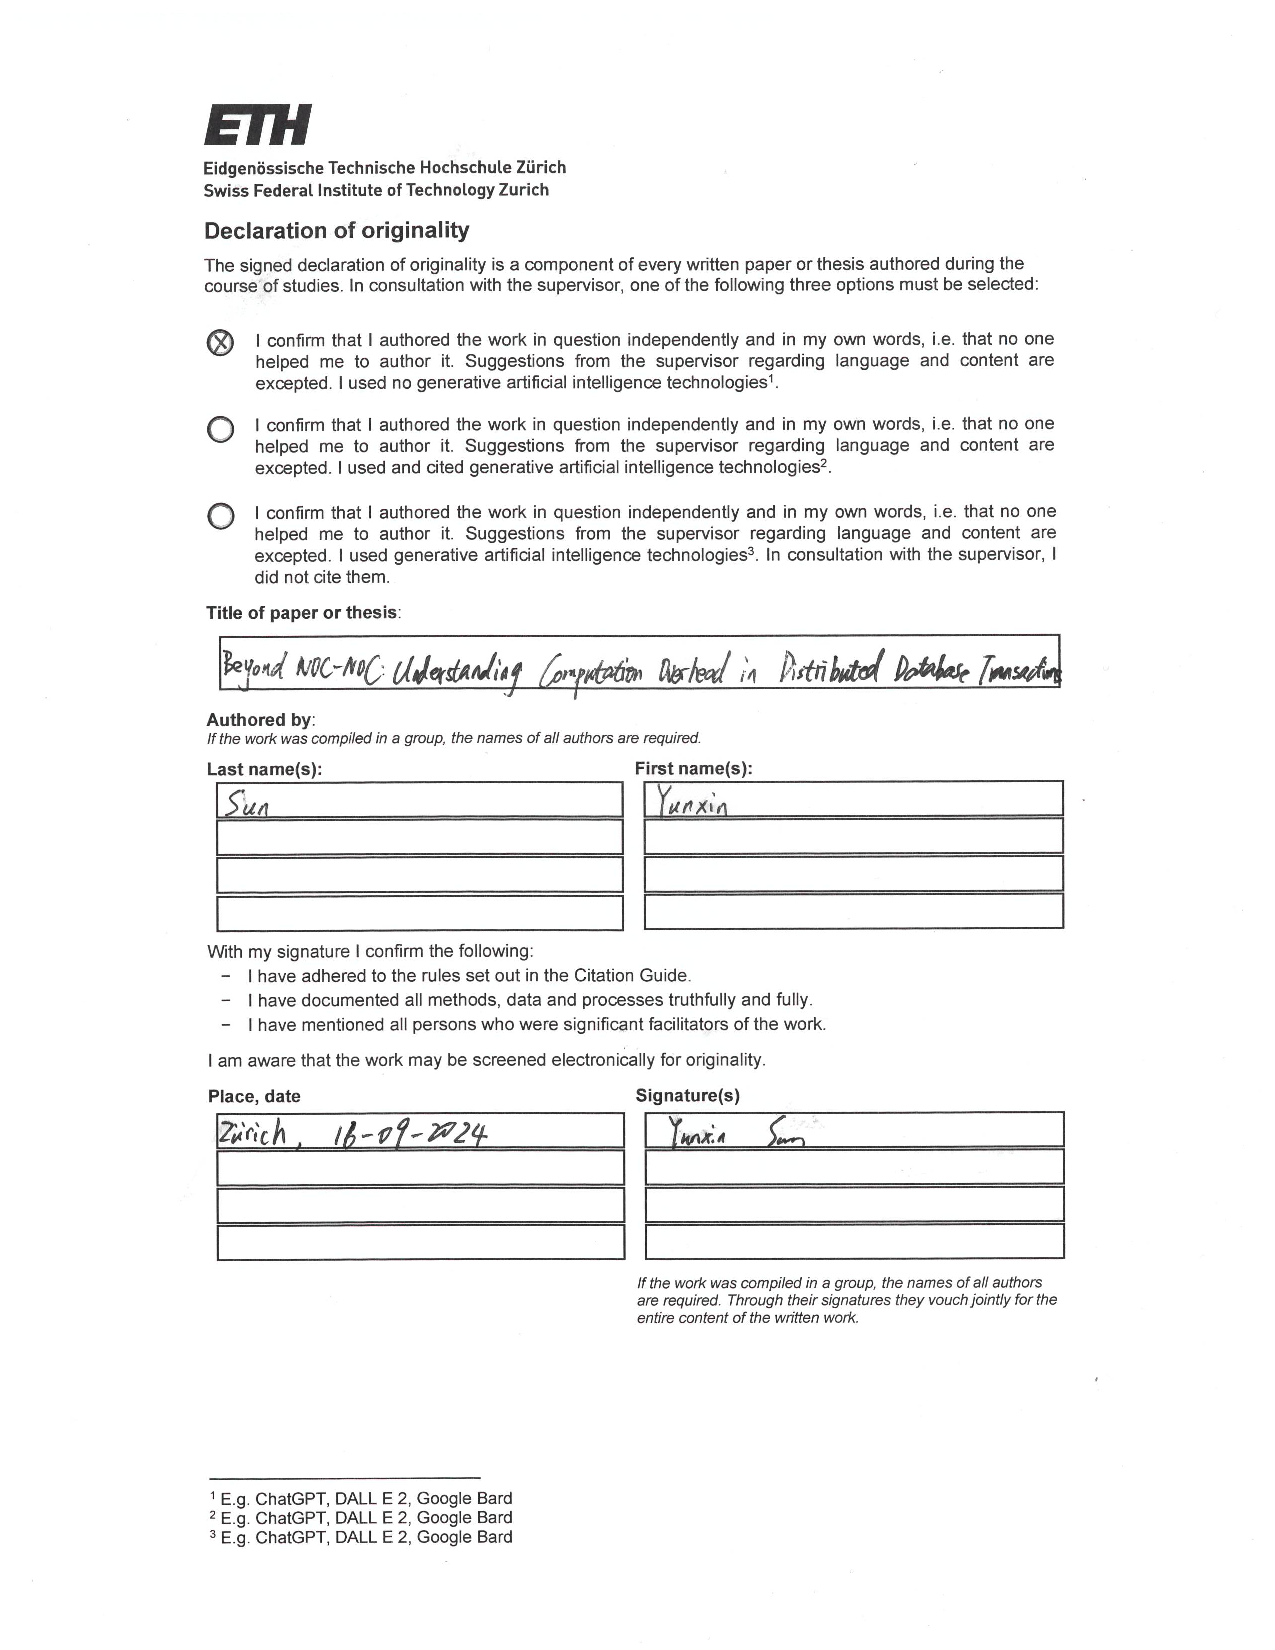
\includepdf[pages={-}]{eth-template/declaration-originality.pdf}

\end{document}
